\documentclass[10pt,twocolumn]{article}
\usepackage[a4paper,margin=1.9cm,top=2.2cm,bottom=2.2cm,columnsep=0.75cm]{geometry}
\usepackage{fontspec}
\setmainfont{Charter}
\setsansfont{Helvetica Neue}
\setmonofont{Menlo}[Scale=0.82]
\newfontfamily\stixfont{STIX Two Text}
\usepackage{microtype}
\usepackage{tikz}
\usetikzlibrary{arrows.meta,positioning,shapes.geometric,calc}
\usepackage{pgfplots}
\pgfplotsset{compat=1.18}
\usepackage{booktabs}
\usepackage{algorithm}
\usepackage{algpseudocode}
\usepackage{amssymb}
\usepackage{gb4e}\noautomath
\usepackage{enumitem}
\setlist{nosep,leftmargin=*}
\usepackage[round,authoryear]{natbib}
\setcitestyle{aysep={},notesep={: }}
\usepackage[hidelinks]{hyperref}
\usepackage{titlesec}
\titleformat{\section}{\large\bfseries\sffamily}{\thesection}{0.7em}{}
\titleformat{\subsection}{\normalsize\bfseries\sffamily}{\thesubsection}{0.6em}{}
\titlespacing*{\section}{0pt}{1.4ex plus .5ex}{0.7ex}
\titlespacing*{\subsection}{0pt}{1.1ex plus .4ex}{0.4ex}
\usepackage{caption}
\captionsetup{font=small,labelfont={bf,sf},labelsep=period}
\usepackage{fancyhdr}
\pagestyle{fancy}\fancyhf{}
\fancyhead[L]{\small\sffamily Källström \& Retourné}
\fancyhead[R]{\small\sffamily Baltmeri: a deterministically synthesised language for the Baltic Sea}
\fancyfoot[C]{\small\thepage}
\renewcommand{\headrulewidth}{0.3pt}
\usepackage{abstract}
\renewcommand{\abstractnamefont}{\sffamily\bfseries\small}
\renewcommand{\abstracttextfont}{\small}
\setlength{\parskip}{0pt}
\hyphenation{Balt-meri}

\title{\sffamily\bfseries\LARGE Baltmeri: Deterministic Synthesis of a Shared Language for the Baltic Sea from the Nine Languages of Its Shores}
\author{\sffamily Martin Källström \and \sffamily Belinda Retourné}
\date{\sffamily\small The Baltmeri Project · September 2026}

\begin{document}
\twocolumn[
\begin{@twocolumnfalse}
\maketitle
\begin{abstract}
\noindent The Baltic Sea is shared by nine languages of four families, none of which names it from the sea's own point of view, and all of which govern it together with limited success: it is the largest human-induced hypoxic area in the world, and regional institutions have not produced a regional identity. We present \textbf{Baltmeri}, a constructed language designed to be the sea's own voice, in which every word is decided by a fixed, repeatable procedure applied to Finnish, Estonian, Latvian, Lithuanian, Polish, Russian, Swedish, Danish and German. Source words are normalised to a common inventory and reduced to consonant skeletons; words already shared across two families are inherited (the Hanse Rule); other content words are assigned to the family with the historically richest vocabulary for their semantic domain; function words and all inflections are decided by one-family-one-vote; ties are broken by the \emph{Visby Queue}, a ranking of the nine languages by distance from the medieval Hanseatic hub, rotating so that no language accumulates decisions. We describe the language's phonology, morphology, syntax and lexicon, and implement the procedure as a deterministic engine with a serialisable tie-break state. Re-deriving the founding Manual's 58 lexical decrees from their nine source forms, the engine reproduces 28; the Domain Rule is 95\% reproducible, and the 30 divergences concentrate in the fill-in of shared words and the counting of ballots, locating exactly where editorial taste survived the algorithm. The seed lexicon is balanced across families, with the three-member Germanic family winning least. We further present a public translator in which a large language model performs only source analysis and dictionary lookup, the engine derives and inflects every word, and a second model call writes an explanation grounded in the engine's trace, so that every Baltmeri word shows its work. We argue, drawing on thalassology, rights-of-nature law and the blue humanities, that an algorithmically synthesised regional language is a legitimate instrument of more-than-human representation: the people around the sea are its citizens, and \emph{Meri er men}, ``the sea is ours'', is true by construction.\par\smallskip\noindent
\textbf{Keywords:} constructed languages; zonal auxiliary languages; Circum-Baltic languages; language contact; consonant skeletons; deterministic lexicogenesis; rights of nature; Baltic Sea; neurosymbolic translation
\end{abstract}
\vspace{1.2em}
\end{@twocolumnfalse}
]

\section{Introduction}\label{sec:intro}

Nine languages are spoken on the shores of the Baltic Sea. They belong to four families---Finnic, Baltic, Slavic and Germanic---that have traded, fished, fought and intermarried across the same water for a thousand years, and yet they mostly cannot understand one another. The sea itself has no name of its own. Germans, Swedes and Danes call it the East Sea (\emph{Ostsee}, \emph{Östersjön}, \emph{Østersøen}); Finns, calquing the Swedish, also call it the East Sea (\emph{Itämeri}) although it lies to their west; Estonians call it the West Sea (\emph{Läänemeri}); Latvians, Lithuanians, Poles and Russians call it the Baltic after a Latin coinage of Adam of Bremen around 1075, whose etymology is itself uncertain \citep{adam1075,jezierski2016}. Each shore names the sea from where it stands. None names it from the sea.

This paper describes \textbf{Baltmeri}, a constructed language designed to be the sea's own: a language whose every word is decided by a fixed, repeatable procedure applied to the nine coastal languages, so that no nation owns it and every nation can hear itself in it. The name is the procedure's first product: \emph{balt-} is shared by Baltic, Slavic and Germanic speakers, and \emph{meri} is what Finns and Estonians call the sea, and what Slavs almost call it (\emph{more}). We present the language's design goals, its phonology, morphology, syntax and lexicon, the algorithm that generates its vocabulary, an evaluation of how faithfully that algorithm reproduces the language's founding text, and a translation system that makes the language usable today.

\subsection{Why the sea needs a voice}
The motivation is ecological before it is linguistic. The Baltic is shallow, brackish and semi-enclosed; its water takes about thirty years to exchange with the North Sea, and its catchment is home to more than 85 million people in fourteen countries \citep{helcom2023}. It is, in the words of \citet{carstensen2014}, ``the largest anthropogenically induced hypoxic area in the world'': oxygen-depleted bottom water has expanded roughly tenfold in a century, from about 5,000 to more than 60,000~km$^2$. HELCOM's holistic assessments found eutrophication affecting 97\% of the sea's area in 2011--2016 and ``no clear signs of recovery'' in 2016--2021, with only four of fifteen commercial fish stocks in good status \citep{helcom2018,helcom2023}. The eastern Baltic cod, once the region's defining fishery, has been under zero-catch advice since 2019 \citep{ices2019}. The Baltic Proper harbour porpoise numbers around five hundred animals whose range crosses the waters of nine states \citep{amundin2022}. Where the coastal states have acted together, the sea has answered: grey seals, reduced to about 3,000 animals in the early 1980s by organochlorine poisoning, were counted at some 42,000 in 2021 \citep{helcomseal}. \citet{reusch2018} draw the general lesson: the Baltic's trend reversals ``could be achieved only by implementing an international, cooperative governance structure transcending its complex multistate policy setting.''

Institutions for that cooperation exist and are old. The Helsinki Convention dates from 1974; the Council of the Baltic Sea States was founded in 1992 \citep{cbss1992}; the EU Strategy for the Baltic Sea Region of 2009 was the Union's first macro-regional strategy \citep{eusbsr2009}; the Baltic Sea Action Plan was adopted in 2007 and renewed in 2021 \citep{helcombsap2021}. Yet identity has not followed institutions. \citet{gotz2016} maps at least eight overlapping regional frameworks and concludes that ``a Baltic Sea identity has barely evolved beyond the circle of an activist elite''; \citet{lehti2003} describe competing, not converging, region-building projects. Historians have long shown that a sea can be written as a subject rather than as the empty space between nations---\citet{braudel1949} for the Mediterranean, \citet{horden2000,horden2006} for the ``new thalassology'', \citet{north2015} for the Baltic as a ``Nordic Mediterranean''---but the people on its shores have few everyday means of experiencing that subject.

Two further developments make the present moment different. First, the law has begun to recognise ecosystems as persons: the Whanganui River in New Zealand \citeyearpar{teawatupua2017}, the Atrato River in Colombia, and, in 2022, the Mar Menor lagoon in Spain, the first European ecosystem with legal personality, established by a citizens' initiative with 639,824 signatures \citep{spain2022,kauffman2021,stone1972}. In the Nordic region, \citet{thiel2024} has proposed an Embassy of the Baltic Sea as ``the first embassy for more-than-human representation in a transnational context'', and describes the human identity it implies as that of a \emph{bioregional citizen belonging to a watershed}. Second, the environmental humanities have supplied a vocabulary for taking such a subject seriously: Haraway's sympoiesis, Latour's Gaia, Neimanis's \emph{hydrocommons}---``we are all bodies of water''---and Steinberg and Peters's ``wet ontology'' of the sea as voluminous, material and continually reforming \citep{haraway2016,latour2017,neimanis2017,steinberg2015}. Neimanis and Åsberg have written specifically of the Baltic, fathoming the chemical weapons dumped in the Gotland Deep \citep{neimanis2017gotland}.

A person needs a voice. \citet{anderson2006} showed that shared print-languages were the substrate on which national communities imagined themselves into being before they existed politically; ecolinguistics has argued that the stories a language makes easy to tell shape how its speakers treat their environment \citep{haugen1972,fill2001,stibbe2021}. Baltmeri is an attempt to run Anderson's mechanism in reverse and on behalf of the sea: to build, deliberately and transparently, a language in which the Baltic is the centre rather than the edge, in which \emph{meri} ``sea'' and \emph{kala} ``fish'' and \emph{hülje} ``seal'' are everyone's words because they were chosen by everyone's languages, and in which the sentence \emph{Meri er men}---``the sea is ours''---is true by construction. We are all citizens of the Baltic; Baltmeri is what those citizens would speak if the sea did the speaking.

\subsection{Why the procedure must be deterministic}
Constructed auxiliary languages have a long history of committees exercising taste \citep{okrent2009,gobbo2020}. For a language meant to belong to nine nations equally, taste is a liability: any choice a Swede or a Pole makes is a choice a Finn or a Latvian can resent. Baltmeri therefore fixes a \emph{procedure} rather than a vocabulary. Two people who follow the Manual with the same nine dictionaries must arrive at the same word; nothing is chosen by preference, and where the nine languages disagree, a fixed voting rule and a rotating tie-break decide. The procedure treats the four families as equal voters, so that the demographic weight of Russian and German cannot swamp Estonian and Latvian, and it breaks ties by distance from Visby on Gotland, the Hanseatic hub in the middle of the sea, so that the tie-break is the sea's geography and not anyone's politics.

Determinism has a second consequence that turns out to be the language's most distinctive feature: every Baltmeri word can \emph{show its work}. Because the derivation is an algorithm, the translator we describe in \S\ref{sec:engine} can display, for every output word, the nine source forms that voted, which family won, and how the tie was broken. In a region where language has so often been an instrument of domination---German as the Hanseatic lingua franca, Swedish, Russian and German as imperial languages in the Baltic provinces \citep{serzant2025,north2015}---a language that is accountable for every one of its words is a small political proposition of its own.

\subsection{Contributions}
\begin{enumerate}
\item A complete description of Baltmeri: source languages and tie-break geography (\S\ref{sec:sources}), phonology and orthography (\S\ref{sec:phonology}), the seven-rule lexicogenesis procedure (\S\ref{sec:procedure}), morphology (\S\ref{sec:morphology}), syntax (\S\ref{sec:syntax}) and lexicon (\S\ref{sec:lexicon}).
\item An implementation of the procedure as a dependency-free, deterministic engine with a serialisable tie-break state, and a reproducibility study in which the engine re-derives the founding Manual's 58 lexical decrees from their nine source forms (\S\ref{sec:eval}). The engine reproduces 28; we classify the 30 divergences and show that they concentrate in one step of one rule.
\item A translation system in which a large language model performs only source-language analysis and dictionary lookup, the engine derives and inflects every Baltmeri word, and a second model call writes an explanation grounded in the engine's trace (\S\ref{sec:engine}), deployed publicly.
\item An argument, developed in \S\ref{sec:discussion}, that an algorithmically synthesised regional language is a legitimate instrument of more-than-human representation, and a candid account of where the Manual's author overrode the algorithm and what that teaches about hand-made versus generated language.
\end{enumerate}

\section{Background and related work}\label{sec:related}

\subsection{The Circum-Baltic contact area}\label{sec:related-cb}
Linguists have studied the languages around the Baltic as an area since \citet{dahl2001} introduced the term ``Circum-Baltic''. The area is unusual in that it is \emph{not} a Sprachbund definable by a shared feature bundle. \citet{koptjevskaja2001} conclude that it is better described as a \emph{contact superposition zone}: many intensive bilateral contacts among small groups of languages, layered over a long period, with no political unification under a single language. \citet{serzant2025} lists twenty-seven isoglosses running through the area; among the very few attested across all of it are a strong tendency toward initial stress (Scandinavian, Latvian, Žemaitian Lithuanian, all Finnic, German, some northern Russian dialects) and German lexical borrowings, ``found in all languages of the area with no exception.'' German during the Hanseatic period was ``probably the only lingua franca to have reached all parts'' of the area. Baltmeri's design reflects both facts: initial stress is adopted by default, and words already shared across families---overwhelmingly Hanseatic in origin---are inherited before any vote takes place (\S\ref{sec:procedure}). The general finding of contact linguistics that intensity of contact, not typological distance, predicts borrowing \citep{thomason1988} explains why a herring can be the same word in Danish and Polish while the two grammars remain alien to each other.

\subsection{The Hanseatic lexical legacy}\label{sec:related-hansa}
The scale of Middle Low German influence on the region is measurable. In Gellerstam's frequency study of the 6,000 most common Swedish words, 24\% are direct German loans and 30\% when German mediation is counted \citep{gellerstam1973,elmevik2012}; \citet{jahr1999} describes Hanseatic merchants settling in Bergen, Stockholm and Copenhagen and Low German entering everyday urban life. German loans are estimated at 22--25\% of Estonian stems \citep{hinderling1981}, and a World Loanword Database template applied to Finnish finds 26\% of the lexicon borrowed, 71\% of it Germanic and chiefly Swedish \citep{cronhamn2018}. Visby was ``the main centre of the Hanseatic League in the Baltic from the 12th to the 14th century'' \citep{unesco1995,dollinger1970}, which is why the Manual anchors its tie-break geography there: the sea's historical hub is the one point no modern state can claim.

\subsection{Zonal and naturalistic constructed languages}\label{sec:related-conlang}
Baltmeri belongs to the family of \emph{zonal} constructed languages, designed for a group of related or neighbouring languages rather than for the world \citep{gobbo2020}. Its closest methodological ancestor is IALA's Interlingua \citep{iala1951}, whose dictionary admitted a word ``when its presence is attested---in corresponding forms and with corresponding meanings---in at least three of the language units'' (Italian, French, English, Spanish/Portuguese, with German and Russian as substitutes), and rendered it in a \emph{prototype} form, ``the nearest common documented or hypothetical ancestor from which all contributing variants can be developed.'' Baltmeri's Hanse Rule is a threshold-plus-prototype rule of the same kind, with two differences: the threshold is counted over families rather than languages, and the form is not a reconstructed prototype but an attested stem chosen by vote. Interslavic is the second ancestor: its six Slavic sub-branches ``are weighed equally in establishing the largest common denominator \ldots\ to prevent any input language from getting undue weight'' \citep{merunka2019,vansteenbergen2016}, exactly the reasoning behind Baltmeri's one-family-one-vote rule; Interslavic's intelligibility surveys (mean 84\% cloze comprehension across 1,822 respondents) show that such a language can be passively understood by speakers who never learned it. Latin-derived and pan-Germanic projects \citep{libert2004} and the broad histories of \citet{okrent2009} and \citet{peterson2015} supply the wider context, from \citet{zamenhof1887} onward. What none of these projects attempted is full determinism: every one of them left the final form of a word to editorial judgement. Baltmeri's contribution to interlinguistics is to remove that judgement and to measure what happens when one does (\S\ref{sec:eval}).

\subsection{Computational comparison of vocabularies}\label{sec:related-comp}
The consonant skeleton at the heart of Baltmeri's procedure has a lineage in computational historical linguistics. \citet{dolgopolsky1986} proposed ten consonant classes such that sound changes within a class are more frequent than changes across classes; the Automated Similarity Judgment Program reduced IPA to 41 sound-class symbols and compared 40-item wordlists across thousands of languages \citep{brown2008,holman2008,wichmann2010,jaeger2018}; \citet{list2012,list2014} refined the classes for phonetic alignment and cognate detection, with accuracies approaching expert judgement \citep{list2017,rama2018}. Baltmeri's eleven classes (Table~\ref{tab:classes}) are coarser than any of these, deliberately: the aim is not to detect cognates but to detect \emph{shared words} regardless of whether they are cognate, borrowed or coincidental, since the sea does not care which. The basic-vocabulary tradition from \citet{swadesh1952,swadesh1955} to the Leipzig--Jakarta list \citep{tadmor2010,haspelmath2009} tells us where to expect agreement: roughly a quarter of an average lexicon is borrowed, but core meanings resist borrowing, so family votes on core vocabulary are least noisy while trade and sea vocabulary is where Hanse words cluster.

\subsection{The sea as subject; language and identity}\label{sec:related-sea}
\S\ref{sec:intro} has set out the ecological and legal context. Here we note the intellectual traditions the design draws on. Thalassology, from \citet{braudel1949} through \citet{horden2000,horden2006} to \citet{north2015} and \citet{kirby2000}, treats a sea as a historical subject with its own rhythms and connections rather than as a container for the nations around it; the medieval Baltic has been studied as an ``imagined community'' in exactly Anderson's sense \citep{jezierski2016,anderson2006}. The blue humanities \citep{mentz2009,gillis2012,steinberg2015} and posthuman feminist work on water \citep{neimanis2017,neimanis2017gotland} argue that the sea is not outside us. Rights-of-nature scholarship, from \citet{stone1972} to \citet{kauffman2021}, shows that legal personhood for ecosystems succeeds where it is embedded in coalitions and has human guardians who speak for the entity, as Te Pou Tupua speaks for the Whanganui \citep{teawatupua2017}. Ecolinguistics \citep{haugen1972,fill2001,stibbe2021} supplies the claim that the stories a language makes available shape ecological conduct; \citet{fishman1989} the link between language and self-definition. Baltmeri operationalises these positions: it gives the guardian something to speak.

\section{Design goals}\label{sec:design}

Baltmeri answers a thought experiment: \emph{what if the sea itself had a grammar, and every word in it were decided by a fixed, repeatable procedure applied to the nine languages spoken on its shores?} The design follows from five commitments.

\paragraph{Determinism.} Two people who follow the Manual with the same nine dictionaries must arrive at the same word. No form is chosen by taste; the only human input is the Manual itself. This is what separates Baltmeri from earlier naturalistic auxiliary languages, whose committees exercised judgement at every entry (\S\ref{sec:related-conlang}).

\paragraph{Equity between families.} The nine languages belong to four families with very unequal speaker numbers (Table~\ref{tab:sources}). Voting therefore happens at the \emph{family} level, one family one vote, so that Germanic's three members, or Russian's demographic weight, cannot swamp the others. Inside a family a fixed sub-ranking (Estonian before Finnish, Latvian before Lithuanian, Polish before Russian, Swedish before Danish before German) settles internal disagreement without rotating.

\paragraph{Rotating tie-breaks.} Ties are unavoidable with four voters. They are broken by the \emph{Visby Queue}, a ranking of the nine languages by the distance from Visby on Gotland---the medieval Hanseatic hub in the middle of the sea---to each language's nearest major coastal city. Whichever language breaks a tie moves to the back of the queue (the \emph{Rota Rule}), so that no single language accumulates decisions.

\paragraph{Inheritance before invention.} Where the languages already agree, Baltmeri inherits (the Hanse Rule). Where they disagree, a content word is assigned to the family with the historically richest vocabulary for its semantic domain. Only function words and inflections are put to a plain vote. New morphology is invented nowhere; every ending is the winner of a vote among existing endings.

\paragraph{Pronounceability across the shore.} The sound inventory is restricted to segments at least three of the nine languages produce comfortably, stress is fixed on the first syllable, and a small set of repair rules eliminates clusters that any coastal speaker would stumble over.

These commitments make Baltmeri a \emph{zonal} constructed language in the sense of \S\ref{sec:related-conlang}, but one whose zone is defined by a body of water rather than by a language family, and whose lexicon is generated by an algorithm rather than curated by hand.

\section{Source languages and the Visby Queue}\label{sec:sources}

\begin{table}[t]
\centering\small
\caption{The nine source languages, their families, and the fixed in-family sub-ranking (left to right). Speaker figures are approximate first-language totals and are given only to motivate family-level voting.}
\label{tab:sources}
\setlength{\tabcolsep}{4pt}
\begin{tabular}{@{}lp{3.1cm}ll@{}}
\toprule
Family & Members, ranked & Abbr. & L1 speakers \\
\midrule
Finnic & Estonian, Finnish & et, fi & $\approx$6 M \\
Baltic & Latvian, Lithuanian & lv, lt & $\approx$4.5 M \\
Slavic & Polish, Russian & pl, ru & $\approx$190 M \\
Germanic & Swedish, Danish, German & sv, da, de & $\approx$110 M \\
\bottomrule
\end{tabular}
\end{table}

The Manual fixes the initial queue as
\begin{quote}
Swedish, Latvian, Lithuanian, Estonian, Finnish, Polish, German, Danish, Russian.
\end{quote}
We checked this ordering against great-circle distances from Visby (57.63°N, 18.30°E) to candidate cities (Table~\ref{tab:visby}). The queue is \emph{approximately} geodesic: Stockholm is nearest and Saint Petersburg farthest, as the Manual has it. Two departures are worth recording. Klaipėda (276~km) is nearer than Riga (357~km), so a strict reading would place Lithuanian before Latvian; and if Kaliningrad (353~km) rather than Saint Petersburg (738~km) were taken as Russia's coastal city, Russian would move from last to third. The Manual's queue is therefore best understood as a \emph{convention fixed by the text}, which the engine treats as an axiom, and not as a quantity to be re-measured. Because the queue rotates on every tie, its \emph{state} after the seed lexicon has been derived---the canonical queue, \S\ref{sec:eval-queue}---depends on the order of derivation, which the Manual also fixes (\S3 to \S11, top to bottom).

\begin{table}[t]
\centering\small
\caption{Great-circle distance from Visby to candidate ``nearest major coastal cities'' (haversine, km). Cities in bold are the ones consistent with the Manual's queue.}
\label{tab:visby}
\begin{tabular}{@{}llr@{}}
\toprule
Language & City & km \\
\midrule
Swedish & \textbf{Stockholm} & 189 \\
Lithuanian & \textbf{Klaipėda} & 276 \\
Russian & Kaliningrad & 353 \\
Latvian & \textbf{Riga} & 357 \\
Polish & \textbf{Gdańsk} & 366 \\
Finnish & Turku & 387 \\
Danish & \textbf{Copenhagen} & 412 \\
Estonian & \textbf{Tallinn} & 425 \\
Finnish & \textbf{Helsinki} & 474 \\
German & \textbf{Rostock} & 551 \\
German & Lübeck & 634 \\
Russian & \textbf{Saint Petersburg} & 738 \\
\bottomrule
\end{tabular}
\end{table}

\begin{figure}[t]
\centering
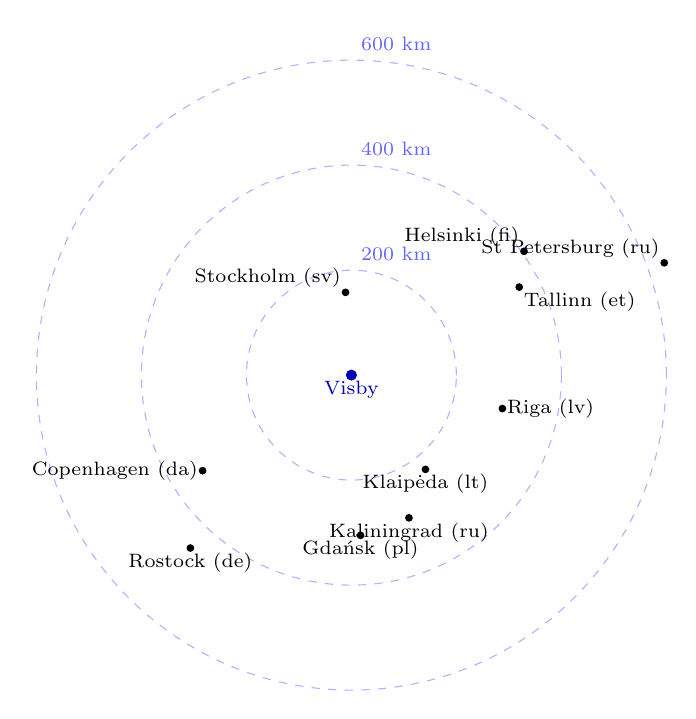
\begin{tikzpicture}[x=0.33cm,y=0.62cm,font=\scriptsize]
  % rings: 200, 400, 600 km  (1 cm = 150 km)
  \foreach \r/\l in {1.333/200 km, 2.667/400 km, 4/600 km} {
    \draw[blue!30,dashed] (0,0) circle [x radius=\r/0.33, y radius=\r/0.62];
    \node[blue!60,anchor=south west] at (0,{\r/0.62}) {\l};
  }
  \fill[blue!70!black] (0,0) circle (2pt) node[anchor=north,inner sep=2pt] {Visby};
  \foreach \lon/\lat/\name/\pos in {
    18.069/59.329/Stockholm (sv)/above left,
    24.105/56.949/Riga (lv)/right,
    21.144/55.703/Klaipėda (lt)/below,
    24.754/59.437/Tallinn (et)/below right,
    24.938/60.170/Helsinki (fi)/above left,
    18.646/54.352/Gdańsk (pl)/below,
    12.099/54.092/Rostock (de)/below,
    12.568/55.676/Copenhagen (da)/left,
    30.335/59.934/St~Petersburg (ru)/above left,
    20.510/54.710/Kaliningrad (ru)/below} {
    \fill[black] ({\lon-18.295},{\lat-57.634}) circle (1.4pt) node[\pos,inner sep=1.5pt] {\name};
  }
\end{tikzpicture}
\caption{The Visby Queue as geography: equirectangular sketch of the nine languages' coastal cities around Visby, with 200, 400 and 600 km rings. Kaliningrad, the Russian city the Manual does not use, is the Russian city the Manual does not use; it would place Russian third.}
\label{fig:visby}
\end{figure}

\section{Phonology and orthography}\label{sec:phonology}

\subsection{Inventory}
Baltmeri admits only sounds that at least three of the nine languages share comfortably. The consonant inventory is
\begin{quote}
p t k b d g m n l r s š z ž v j h ts dz
\end{quote}
to which the derived lexicon adds \emph{č} (from Polish \emph{cz}, Baltic \emph{č}, Russian \emph{ч}: \emph{četri} ``four'', \emph{odpočiv-} ``rest'') and \emph{f} in a handful of Germanic-won forms (\emph{fem} ``five''). Both are tolerated as marginal segments. The vowels are \emph{a e i o u ä ö ü}; length is phonemic and written by doubling (\emph{jää} ``ice'', \emph{lääs} ``west'', \emph{juus} ``you (pl.)''). Orthography is one letter per segment, with the Estonian--Latvian--Lithuanian convention for \emph{š ž č} and the Finnish--Estonian--German--Swedish convention for the front rounded vowels; no source language has to learn a new letter shape.

\subsection{Stress}
Stress falls on the first syllable. Finnish, Estonian and Latvian have fixed initial stress; Lithuanian native words and most German and Swedish simplex words lean that way; no family strongly objects. Initial stress interacts with the morphology: since all inflection is suffixal, the stressed stem is never obscured by an ending.

\subsection{The Normalization Table}\label{sec:normalization}
Every source word passes through an ordered rewrite table before it takes part in any decision (Table~\ref{tab:normalization}). The table maps each language's orthography onto the Baltmeri inventory. Its purpose is not phonetic accuracy but \emph{comparability}: after normalization, Swedish \emph{båt}, Danish \emph{båd}, German \emph{Boot} and Estonian \emph{paat} can be recognised as one word. Suprasegmentals that no other family shares---Danish \emph{stød}, Swedish pitch accent, Russian vowel reduction---are ignored, and voiced final obstruents stay voiced (\emph{duž} ``big'').

\begin{table}[t]
\centering\small
\caption{The Normalization Table (\S2 of the Manual), as implemented. Rules apply in order within a language.}
\label{tab:normalization}
\setlength{\tabcolsep}{4pt}
\begin{tabular}{@{}p{3.4cm}p{1.5cm}p{2.5cm}@{}}
\toprule
Source feature & Becomes & Example \\
\midrule
sv/da \emph{å}; fi/et \emph{oo} & o / oo & \emph{båt} $\rightarrow$ bot \\
sv/de \emph{y}; fi/et \emph{y/ü}; de \emph{ü} & ü & \emph{yksi} $\rightarrow$ üksi \\
et \emph{õ} & ö & \emph{võrk} $\rightarrow$ vörk \\
lv/lt macrons, nasal vowels & doubled vowel & \emph{jūs} $\rightarrow$ juus \\
pl \emph{ę, ą} before C & en, an (em, am before b/p) & \emph{głęboki} $\rightarrow$ glembok \\
pl \emph{cz}, ru \emph{ч} & č & \emph{cztery} $\rightarrow$ čteri \\
pl \emph{sz}, ru \emph{ш} & š & \emph{szary} $\rightarrow$ šar \\
pl \emph{ż/rz}, ru \emph{ж} & ž & \emph{żeglować} $\rightarrow$ žegl- \\
pl \emph{ł}, ru dark \emph{l} & l & \emph{pływać} $\rightarrow$ plav- \\
pl/ru palatalisation (\emph{ś ń ź ь}) & dropped & \emph{sól} $\rightarrow$ sol \\
de \emph{ch, sch} & h, š & \emph{Sprache} $\rightarrow$ sprahe \\
de \emph{z, tz}; lv/lt \emph{c} & ts & \emph{Salz} $\rightarrow$ salts \\
lv \emph{dz}, lt \emph{dž} & dz & \emph{dzintars} $\rightarrow$ dzintar \\
Geminates & single & \emph{sill} $\rightarrow$ sil \\
Multi-word citations & fused & \emph{i går} $\rightarrow$ igor \\
\bottomrule
\end{tabular}
\end{table}

\subsection{Consonant skeletons}\label{sec:skeleton}
The currency of the whole system is the \emph{consonant skeleton}: the sequence of a normalized word's consonants with voicing and palatalisation ignored. We group segments into eleven classes (Table~\ref{tab:classes}). Affricates fold into their stop, so Polish \emph{śledź} ($\rightarrow$ \emph{sledz}) and Danish \emph{sild} share the skeleton S-L-T and count as ``the same word'' even though no listener would guess it by ear. The skeleton is a deliberately coarse similarity measure in the tradition of sound-class comparison in computational historical linguistics (\S\ref{sec:related-comp}); it trades phonetic detail for robustness to the vowel changes, gradation and umlaut that separate cognates and old loans around the Baltic.

\begin{table}[t]
\centering\small
\caption{Skeleton classes. \emph{j} is treated as a semivowel for cluster purposes (\S\ref{sec:repair}).}
\label{tab:classes}
\begin{tabular}{@{}ll@{}}
\toprule
Class & Segments \\
\midrule
P & p b f \\
T & t d ts dz \\
K & k g \\
S & s z š ž \\
Č & č \\
M, N, L, R, V, J, H & m; n; l; r; v; j; h \\
\bottomrule
\end{tabular}
\end{table}

Two skeletons \emph{match} if they have the same length and differ in at most one position. We restrict the one-position tolerance to skeletons of three or more consonants: for one- and two-consonant skeletons a differing position would match almost anything (S-L ``salt'' would match S-R ``island''), and the Manual's own examples of tolerated difference (\emph{dzintar}/\emph{gintar}/\emph{jantar}, \emph{četri}/\emph{keturi}) all involve three or four consonants. This threshold is the single most consequential interpretive decision in the implementation, and we return to it in \S\ref{sec:eval}.

\section{The synthesis procedure}\label{sec:procedure}

Every Baltmeri word is the output of the procedure in Algorithm~\ref{alg:synth}, run on a \emph{concept}: an English gloss, a part of speech, a semantic domain, and the first dictionary translation in each of the nine languages. The rules are tried in order and the first that yields an answer wins. Figure~\ref{fig:flow} shows the same procedure as a decision path.

\begin{algorithm}[t]
\caption{Lexicogenesis: Rules 0--6 of the Manual.}
\label{alg:synth}
\begin{algorithmic}[1]
\Require concept $c$ with sources $s_\ell$ for $\ell \in L$; queue $Q$; taken forms $T$
\State \textbf{Gather:} for each $\ell$: strip citation ending, normalize, $\sigma_\ell \gets$ skeleton \Comment{Rule 0}
\State cluster the $\sigma_\ell$ by \textsc{match}; let $C^\ast$ be the cluster spanning most families
\If{$C^\ast$ spans $\geq 2$ families} \Comment{Rule 1, Hanse}
  \State each family in $C^\ast$ nominates its front-ranked member's stem
  \State $w \gets$ plurality; ties broken by $Q.\textsc{break}$ (winner rotates to back)
\ElsIf{$c$ is a content word with domain $d$} \Comment{Rule 2, Domain}
  \State $F \gets \textsc{family}(d)$; $w \gets$ stem of the front-ranked member of $F$ with a form
\Else \Comment{Rule 3, Family Vote}
  \State each family casts a ballot iff its members' skeletons match (else abstains)
  \State pool ballots by \textsc{match}; $w \gets$ plurality; ties by $Q.\textsc{break}$
  \If{every family abstained} $w \gets$ form of $Q.\textsc{fallback}$ \Comment{Rule 4}
  \EndIf
\EndIf
\If{$w \in T$} $w \gets$ next candidate not in $T$ \Comment{Rule 5, Collision}
\EndIf
\State $T \gets T \cup \{w\}$; \Return $w$ (Repair, Rule 6, is applied when suffixes attach)
\end{algorithmic}
\end{algorithm}

\begin{figure}[t]
\centering
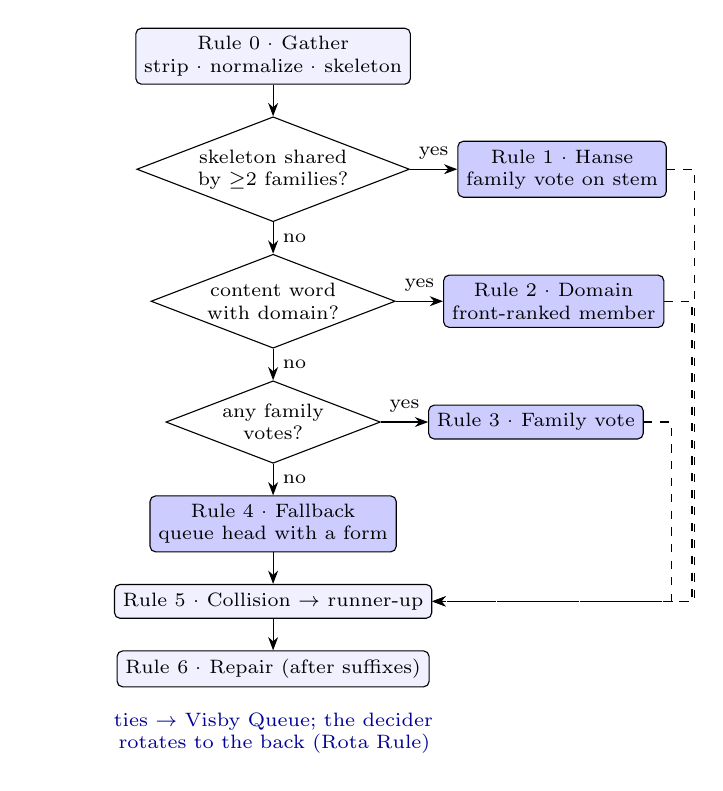
\begin{tikzpicture}[font=\scriptsize,node distance=4mm,
  box/.style={draw,rounded corners=2pt,fill=blue!6,minimum width=2.4cm,align=center,inner sep=3pt},
  dec/.style={draw,diamond,aspect=2.6,fill=white,align=center,inner sep=1pt},
  res/.style={draw,fill=blue!20,rounded corners=2pt,align=center,inner sep=3pt},
  >=Stealth]
  \node[box] (g) {Rule 0 · Gather\\strip · normalize · skeleton};
  \node[dec,below=of g] (h) {skeleton shared\\by $\geq$2 families?};
  \node[res,right=6mm of h] (ho) {Rule 1 · Hanse\\family vote on stem};
  \node[dec,below=of h] (d) {content word\\with domain?};
  \node[res,right=6mm of d] (do) {Rule 2 · Domain\\front-ranked member};
  \node[dec,below=of d] (v) {any family\\votes?};
  \node[res,right=6mm of v] (vo) {Rule 3 · Family vote};
  \node[res,below=of v] (f) {Rule 4 · Fallback\\queue head with a form};
  \node[box,below=of f] (c) {Rule 5 · Collision $\rightarrow$ runner-up};
  \node[box,below=of c] (r) {Rule 6 · Repair (after suffixes)};
  \draw[->] (g)--(h); \draw[->] (h)--node[above]{yes}(ho); \draw[->] (h)--node[right]{no}(d);
  \draw[->] (d)--node[above]{yes}(do); \draw[->] (d)--node[right]{no}(v);
  \draw[->] (v)--node[above]{yes}(vo); \draw[->] (v)--node[right]{no}(f);
  \draw[->] (f)--(c); \draw[->] (c)--(r);
  \draw[->,dashed] (ho.east) -- ++(0.35,0) |- (c.east);
  \draw[->,dashed] (do.east) -- ++(0.35,0) |- (c.east);
  \draw[->,dashed] (vo.east) -- ++(0.35,0) |- (c.east);
  \node[below=2mm of r,align=center,text width=6cm,text=blue!60!black] {ties $\rightarrow$ Visby Queue; the decider rotates to the back (Rota Rule)};
\end{tikzpicture}
\caption{The decision path of the synthesis procedure.}
\label{fig:flow}
\end{figure}

\subsection{Rule 0: Gather}
Citation-form endings are stripped before normalization so that they are still recognisable: Swedish/Danish infinitive \emph{-a/-e}, German \emph{-en}, Finnish \emph{-a/-ä}, Estonian \emph{-ma}, Latvian \emph{-t}, Lithuanian \emph{-ti}, Polish \emph{-ć} with its theme vowel, Russian \emph{-ть}; nominal endings Latvian \emph{-s/-a}, Lithuanian \emph{-as/-is/-a}, and Polish/Russian gender vowels. Stems keep at least two letters, so Polish \emph{być} yields \emph{by-} rather than \emph{b-}. Polish \emph{kochać} $\rightarrow$ \emph{koch} $\rightarrow$ \emph{koh}; \emph{odpoczywać} $\rightarrow$ \emph{odpočiv}; Latvian \emph{pelēks} $\rightarrow$ \emph{peleek}.

\subsection{Rule 1: the Hanse Rule}
If the same skeleton appears in two or more families, the concept is a \emph{Hanse word}---something that has already crossed the sea on its own---and Baltmeri takes it. \emph{Herring}: Danish \emph{sild}, Polish \emph{śledź}, Russian \emph{сельдь} all give S-L-T, and Latvian \emph{siļķe}/Lithuanian \emph{silkė} give S-L-K, one position away; three families share the skeleton. \emph{Salt}: Finnish \emph{suola}, Estonian \emph{sool}, Polish \emph{sól}, Russian \emph{соль} share S-L. \emph{Amber}: Latvian \emph{dzintars}, Lithuanian \emph{gintaras}, Russian \emph{янтарь} share T/K/J-N-T-R with one differing onset.

The Manual says the vowels and any disputed consonant are ``filled in by family vote, ties by the Visby Queue''. We implement this as a vote on whole stems: each supporting family nominates its front-ranked member's normalized stem, plurality wins, ties go to the queue. An earlier implementation voted position by position (each vowel slot and each disputed consonant separately) and produced blends no coastal speaker would recognise (\emph{muur} for ``sea'' from \emph{meri}/\emph{mor}/\emph{meer}); whole-stem voting keeps every Hanse word a word that actually exists somewhere on the shore.

\subsection{Rule 2: the Domain Rule}
Content words with no shared skeleton are assigned to a family by semantic domain, on the historical logic of who has the oldest and richest vocabulary for it (Table~\ref{tab:domains}). Inside the family the fixed sub-ranking decides: Estonian before Finnish gives \emph{räim} ``Baltic herring'' (fi \emph{silakka}), \emph{suvi} ``summer'' (fi \emph{kesä}), \emph{kalju} ``rock'' (fi \emph{kallio}); Polish before Russian gives \emph{duž} ``big'' (ru \emph{большой}), \emph{koh-} ``love'' (ru \emph{любить}).

\begin{table}[t]
\centering\small
\caption{Semantic domains and the family that owns them (Rule 2).}
\label{tab:domains}
\begin{tabular}{@{}p{4.2cm}l@{}}
\toprule
Domain & Family \\
\midrule
Sea, fish and sea animals, weather, seasons, landscape, parts of boats & Finnic \\
Body, kinship, colours, farm, forest & Baltic \\
Trade, tools, town, law, money, abstract nouns & Germanic \\
Verbs of action, motion and emotion; adjectives of quality & Slavic \\
\bottomrule
\end{tabular}
\end{table}

\subsection{Rules 3 and 4: Family Vote and Fallback}
Pronouns, conjunctions, particles, numerals and all inflectional endings are decided by family vote. A family votes only if its members agree (same skeleton, one differing position allowed); otherwise it abstains. Most votes wins; ties go to the queue. \emph{Two}: D-V in Baltic (\emph{divi}), Slavic (\emph{dva}) and Germanic (\emph{två}) $\rightarrow$ \emph{dva}. \emph{Three}: T-R everywhere except Finnic $\rightarrow$ \emph{tri}. If every family abstains, the word is taken from the first language in the current queue that has a form at all, and that language moves to the back: the yes/no particle \emph{li} is Russian's, in Russian's post-verbal position, because Estonian \emph{kas}, Latvian \emph{vai}, Lithuanian \emph{ar} and Polish \emph{czy} agree on nothing.

\subsection{Rule 5: Collision}
If two concepts produce the same form, the one derived later takes the runner-up from its own vote. \emph{And}: Finnic \emph{ja} and Slavic \emph{i} tie, the queue favours Estonian, but \emph{ja} already means ``I'' (\S\ref{sec:pronouns}), so ``and'' is \emph{i}. Collisions are checked against every form coined so far, including new words derived at translation time, so the lexicon stays injective.

\subsection{Rule 6: Repair}\label{sec:repair}
Repair runs once all suffixes are attached and touches only clusters created by attaching a suffix; a cluster inside a derived stem (\emph{Baltmeri}, \emph{tursk}) is part of the word. (i) Identical adjacent consonants merge: \emph{lääs-ste} $\rightarrow$ \emph{lääste}. (ii) A cluster of three or more consonants across the boundary takes an epenthetic \emph{i}: before a final single-consonant suffix (\emph{vid-s-t} $\rightarrow$ \emph{vidsit}), otherwise right after the stem (\emph{vid-l-me} $\rightarrow$ \emph{vidilme}, \emph{pospolit-st} $\rightarrow$ \emph{pospolitist}). (iii) A word-final two-consonant cluster is allowed only if its first consonant is a sonorant or \emph{s} (\emph{talv}, \emph{sort}, \emph{bust}); otherwise \emph{i} is inserted (\emph{vid-t} $\rightarrow$ \emph{vidit}, \emph{duž-m} $\rightarrow$ \emph{dužim}); a final \emph{-s} is tolerated (\emph{vids}, \emph{bus}). (iv) Suffixes consisting of a single obstruent carry a supporting \emph{-e} in the tables (inessive \emph{-se}, allative \emph{-le}, infinitive \emph{-te}). \emph{j} is a semivowel and never forms a cluster (\emph{žeglja} ``sailor'', \emph{kalaja} ``fisher'').

\subsection{Worked example: \emph{herring}}
Table~\ref{tab:herring} traces the full derivation. Nine forms are gathered and normalized; five of them (Latvian, Lithuanian, Polish, Russian, Danish) fall into one skeleton cluster spanning three families, so the Hanse Rule fires. Baltic nominates \emph{silk}, Slavic \emph{sledz}, Germanic \emph{sild}: a three-way tie. The initial queue puts Swedish first, but Swedish \emph{sill} (S-L) is not in the cluster; Latvian is next and is, so the engine's verdict is \emph{silk} and Latvian rotates to the back. The Manual, however, decrees \emph{sild}. This is the pattern behind most of the divergences reported in \S\ref{sec:eval}: the algorithm and the Manual's author agree on \emph{which} words are Hanse words and \emph{who} owns a domain, and disagree on the last step of filling in a shared skeleton.

\begin{table}[t]
\centering\small
\caption{Derivation trace for \emph{herring}. Skeleton cluster members are marked $\bullet$.}
\label{tab:herring}
\begin{tabular}{@{}llllc@{}}
\toprule
Lang. & Source & Stem & Skeleton & \\
\midrule
fi & silli & sili & S-L & \\
et & heeringas & heeringas & H-R-N-K-S & \\
lv & siļķe & silk & S-L-K & $\bullet$ \\
lt & silkė & silk & S-L-K & $\bullet$ \\
pl & śledź & sledz & S-L-T & $\bullet$ \\
ru & сельдь & seld & S-L-T & $\bullet$ \\
sv & sill & sil & S-L & \\
da & sild & sild & S-L-T & $\bullet$ \\
de & Hering & hering & H-R-N-K & \\
\midrule
\multicolumn{5}{@{}p{7.2cm}@{}}{Rule 1: cluster spans Baltic, Slavic, Germanic. Ballots: \emph{silk}, \emph{sledz}, \emph{sild}. Tie $\rightarrow$ queue (sv, \textbf{lv}, lt, et, fi, pl, de, da, ru) $\rightarrow$ Latvian $\rightarrow$ \emph{silk}; Latvian to the back. Manual decree: \emph{sild}.} \\
\bottomrule
\end{tabular}
\end{table}

\section{Morphology}\label{sec:morphology}

All inflection is suffixal, agglutinative and stress-neutral. Every ending is itself the product of a family vote recorded in the Manual, so the grammar is derived by the same procedure as the lexicon.

\subsection{Nouns}\label{sec:nouns}
\paragraph{No gender.} Finnic has none; Baltic, Slavic and Germanic disagree with one another about which nouns are what. Gender assignment cannot be made deterministic across the nine and is abolished. This is also the honest outcome of the vote: three gendered families with three incompatible systems cannot agree on a form.

\paragraph{No articles.} Finnic, Baltic and Slavic have none: three votes to one.

\paragraph{Plural \emph{-i}.} Baltic (lv \emph{-i}, lt \emph{-ai/-iai}) and Slavic (\emph{-i/-y}) agree on the vowel; Finnic \emph{-t/-d} and Germanic \emph{-er/-e/-en} each cast one vote: 2--1--1. \emph{kala} $\rightarrow$ \emph{kalai}, \emph{hülje} $\rightarrow$ \emph{hüljei}, \emph{sort} $\rightarrow$ \emph{sorti}.

\paragraph{Seven cases.} Finnic's rich case system and the Baltic--Slavic middle ground produce seven cases (Table~\ref{tab:cases}); Germanic contributes little because its cases are mostly gone. Plural and case stack, stem + \emph{-i} + case: \emph{kalju-i-l} ``on the rocks'', \emph{Baltmeri-se} ``in the Baltic''. The accusative plural is identical to the nominative plural, as for inanimates in Slavic and generally in Finnic and Germanic. Compounds are head-final and written solid, as in every source language: \emph{peleekhülje} ``grey seal'' (the species) against \emph{peleek hülje} ``a seal that happens to be grey''.

\begin{table}[t]
\centering\small
\caption{Noun cases and the votes that produced them.}
\label{tab:cases}
\setlength{\tabcolsep}{4pt}
\begin{tabular}{@{}llp{1.8cm}p{2.9cm}@{}}
\toprule
Case & Ending & Meaning & Source of the vote \\
\midrule
Nominative & -Ø & subject & unanimous \\
Genitive & -n & of, 's & Finnic -n, Germanic -s, Slavic -a tie $\rightarrow$ Estonian \\
Accusative & -a & direct object & all abstain $\rightarrow$ Fallback $\rightarrow$ Lithuanian -ą \\
Inessive & -se & in, inside & only Finnic has a suffix (-ssa/-s) \\
Adessive & -l & on, at; also \emph{when} & Finnic -lla/-l \\
Elative & -ste & from, out of & Finnic -sta/-st \\
Allative & -le & to, onto & Finnic -lle/-le \\
\bottomrule
\end{tabular}
\end{table}

\subsection{Adjectives, comparison, adverbs}
Adjectives are bare stems and precede the noun (all nine put adjectives first). They agree in number only---Germanic-style partial agreement, since the full-agreement families cannot agree on \emph{how}: \emph{duž kala} ``big fish'', \emph{duži kalai} ``big fish (pl.)''. Comparative \emph{-m} (Germanic \emph{-er/-are}, Slavic \emph{-ejš/-sz}, Finnic \emph{-mpi/-m}, three-way tie $\rightarrow$ Estonian): \emph{dužim} ``bigger''. Superlative \emph{-st} (Germanic \emph{-st}, Slavic \emph{naj-} tie $\rightarrow$ Swedish): \emph{pospolitist} ``most common''. Adverb \emph{-t} (Finnic and Germanic agree on the dental, 2--1--1): \emph{dužit} ``greatly''. Derived adjective \emph{-ne} (Finnic \emph{-(i)nen/-ne}, Slavic \emph{-ny}): \emph{solne} ``salty'', \emph{zimne} ``cold''.

\subsection{Pronouns and numerals}\label{sec:pronouns}
Table~\ref{tab:pronouns} lists the personal pronouns and the numerals one to five, each with its vote. Genitives are \emph{jan, tun, hanen, men, juusen, den}. The third person is genderless, like Finnish \emph{hän}. The numerals alone show the Rota Rule at work: five words, five different tie-break winners (Finnish, plurality, plurality, Baltic--Slavic, Danish). Six to ten are derived by the same procedure and have no manual decree: \emph{seši, septini, ota, dzevents, desmit}.

\begin{table}[t]
\centering\small
\caption{Pronouns and lower numerals with their votes.}
\label{tab:pronouns}
\begin{tabular}{@{}llp{4.6cm}@{}}
\toprule
& Baltmeri & Vote \\
\midrule
I & ja & pl/ru \emph{ja}, sv \emph{jag}, da \emph{jeg}: J in two families \\
you & tu & T-onset in three families; \emph{u} beats \emph{y} \\
he/she/it & han & fi \emph{hän} + sv/da \emph{han}: H-N in two families \\
we & me & M-onset in three families; Baltic final -s dropped \\
you (pl.) & juus & Finnic \emph{te}, Baltic \emph{jūs}, Slavic \emph{vy} tie $\rightarrow$ Latvian \\
they & de & Slavic \emph{oni}, Germanic \emph{de} tie $\rightarrow$ Swedish \\
\midrule
1 & üks & four-way tie $\rightarrow$ Finnish \emph{yksi} \\
2 & dva & D-V in Baltic, Slavic, Germanic \\
3 & tri & T-R everywhere except Finnic \\
4 & četri & Baltic + Slavic, one differing position \\
5 & fem & Slavic vs Germanic tie $\rightarrow$ Danish \\
\bottomrule
\end{tabular}
\end{table}

\subsection{Verbs}
The infinitive is \emph{-te}: Baltic \emph{-t/-ti} and Slavic \emph{-ć/-t'} agree on the dental, plus the supporting \emph{-e}. Finnic, Baltic and Slavic all inflect for person; only Swedish and Danish do not, so 3--1, Baltmeri inflects. Each slot was voted separately (Table~\ref{tab:verbs}). The third person is unmarked for number, Scandinavian-style; the plural subject carries the plural. Past \emph{-l-} (Germanic dental vs Slavic \emph{-l} tie $\rightarrow$ Polish) and future \emph{-s-} (Baltic is the only family with a synthetic future, and the Manual prefers a suffix to a helper verb wherever one exists) are inserted between stem and person ending. Negation is \emph{ne} before the verb (Baltic \emph{ne-}, Slavic \emph{nie/ne}); after the copula, \emph{ne} precedes the predicate (\emph{Baltmeri er ne glembok meri} ``the Baltic is not a deep sea''). The answer-word ``no'' is \emph{nei} (Germanic \emph{nej} + Finnic \emph{ei}). The copula is suppletive, as in all nine languages (Table~\ref{tab:copula}): present \emph{es-} is a Hanse word (lv \emph{esmu}, lt \emph{esu}, pl \emph{jestem}); the third person \emph{er} is a separate vote (lv \emph{ir}, lt \emph{yra}, sv \emph{är}, da \emph{er}).

\begin{table}[t]
\centering\small
\caption{Person endings and the full regular paradigm of \emph{vidte} ``to see''. Forms in italics show Repair (\S\ref{sec:repair}).}
\label{tab:verbs}
\begin{tabular}{@{}llp{2.6cm}@{}}
\toprule
& Ending & Vote \\
\midrule
1sg & -u & lv, lt, ru \emph{-u}: two families \\
2sg & -t & Finnic \emph{-t/-d}, Baltic \emph{-i}, Slavic \emph{-š} tie $\rightarrow$ Finnish \\
3sg & -Ø & lv, pl, sv, da all zero \\
1pl & -me & M in all four families \\
2pl & -te & T in all four families \\
3pl & -Ø & Finnic \emph{-vat} vs Germanic Ø tie $\rightarrow$ Danish \\
\bottomrule
\end{tabular}

\medskip
\begin{tabular}{@{}llll@{}}
\toprule
& Present & Past (-l-) & Future (-s-) \\
\midrule
ja & vidu & vidlu & vidsu \\
tu & \emph{vidit} & \emph{vidlit} & \emph{vidsit} \\
han / de & vid & \emph{vidil} & vids \\
me & vidme & \emph{vidilme} & \emph{vidisme} \\
juus & vidte & \emph{vidilte} & \emph{vidiste} \\
\bottomrule
\end{tabular}
\end{table}

\begin{table}[t]
\centering\small
\caption{The copula \emph{bute} ``to be''.}
\label{tab:copula}
\begin{tabular}{@{}llll@{}}
\toprule
& Present & Past & Future \\
\midrule
ja & esu & bulu & busu \\
tu & est & bulit & bust \\
han / de & er & bul & bus \\
me & esme & bulme & busme \\
juus & este & bulte & buste \\
\bottomrule
\end{tabular}
\end{table}

\subsection{Derivation}
Four productive suffixes were voted: \emph{-us} abstract noun (Finnic \emph{-us}, Baltic \emph{-um(a)s}): \emph{dužus} ``size''; \emph{-ja} agent (Finnic \emph{-ja}, Baltic \emph{-ējs/-ėjas}): \emph{kalaja} ``fisher'', \emph{žeglja} ``sailor''; \emph{-ka} diminutive (Slavic \emph{-ek/-ka}, Estonian \emph{-ke}): \emph{kalaka} ``little fish''; \emph{-ne} adjective from noun: \emph{solne} ``salty''. Derived stems inflect like their base: \emph{dužusi} ``sizes'', \emph{kalajai} ``fishers''.

\section{Syntax}\label{sec:syntax}

Baltmeri syntax was decided by the same votes as its morphology, and it is deliberately plain.

\paragraph{SVO, no inversion.} All nine languages are SVO at rest \citep{dryer2013}; only Germanic has verb-second \citep{holmberg2015}, and it loses 3--1. There is no inversion, ever: a fronted time adverb leaves subject and verb in place, \emph{Home me plavisme} ``tomorrow we will swim'', where Swedish or German would invert.

\paragraph{Modifiers precede.} Adjective before noun, genitive before noun (\emph{Baltmerin kala} ``the sea's fish''), numeral before noun. Quantifiers take the plain plural (\emph{daug kalai} ``many fish''); the Finnic partitive lost.

\paragraph{Place before time.} Adverbial phrases go to the end of the clause, place before time (the Slavic and Germanic order; Finnic is flexible): \emph{odpočiv kaljuil suvil} ``rest on the rocks in summer''.

\paragraph{Existence.} Existence is expressed with \emph{er} and the adessive: \emph{Meril er jää} ``there is ice on the sea''.

\paragraph{Negation and questions.} \emph{Ne} precedes the verb, or the predicate after the copula; the yes/no particle \emph{li} follows the verb: \emph{Tu kohit li meria?} ``do you love the sea?''.

\subsection{Example sentences}
The Manual's three founding sentences, glossed. Abbreviations: \textsc{gen} genitive, \textsc{acc} accusative, \textsc{ine} inessive, \textsc{ade} adessive, \textsc{ela} elative, \textsc{all} allative, \textsc{pl} plural, \textsc{sup} superlative, \textsc{fut} future, \textsc{q} question particle.

\begin{exe}
\ex \gll Baltmeri-n kala er daug sort-i i dužus-i. \\
Baltic-\textsc{gen} fish is many sort-\textsc{pl} and size-\textsc{pl} \\
\glt `The fish in the Baltic Sea come in many varieties and sizes.'
\ex \gll Peleek-hülje-i odpočiv kalju-i-l suvi-l. \\
grey-seal-\textsc{pl} rest.3 rock-\textsc{pl}-\textsc{ade} summer-\textsc{ade} \\
\glt `Grey seals rest on the rocks in summer.'
\ex \gll Räim er pospolit-ist kala Baltmeri-se. \\
Baltic.herring is common-\textsc{sup} fish Baltic-\textsc{ine} \\
\glt `Herring is the most common fish in the Baltic Sea.'
\ex \gll Ja vid-u kala-a vesi-se. \\
I see-1\textsc{sg} fish-\textsc{acc} water-\textsc{ine} \\
\glt `I see a fish in the water.'
\ex \gll Tu koh-it li meri-a? \\
you love-2\textsc{sg} \textsc{q} sea-\textsc{acc} \\
\glt `Do you love the sea?'
\ex \gll Home me žegl-is-me Gotland-ile boot-se. \\
tomorrow we sail-\textsc{fut}-1\textsc{pl} Gotland-\textsc{all} boat-\textsc{ine} \\
\glt `Tomorrow we sail to Gotland in a boat.'
\ex \gll Ne plav-it talv-il! \\
not swim-2\textsc{sg} winter-\textsc{ade} \\
\glt `Don't swim in winter!'
\ex \gll Üks duž kala er duž-im kui tri mal-i. \\
one big fish is big-\textsc{comp} than three small-\textsc{pl} \\
\glt `One big fish is bigger than three small ones.'
\end{exe}

All eight sentences are reproduced verbatim by the engine from a hand-written analysis (\S\ref{sec:eval-sent}), with one exception discussed there.

\subsection{A text}
The Manual closes its grammar with a short text, given here in Baltmeri with a translation; new words it introduces are listed in Appendix~\ref{app:lexicon}.

\begin{quote}\small
\textbf{Baltmeri}\\
Baltmeri er ne glembok meri. Baltmerin vesi er ne müket solne, i talvil meril er jää. Daug kalai plav Baltmerise: räim, sild, tursk i lohi. Peleekhüljei ži saaril i kaljuil, i suvil de odpočiv päivel.

Kalajai lov räima sügisl. Vakar de vidil daug hüljei meril. Home me žeglisme Gotlandile, i ja vidsu dzintara rannal.

Ja kohu Baltmeria. Meri er zimne, ne glembok, i ne müket solne---ale meri er men.
\end{quote}
\begin{quote}\small\itshape
The Baltic is not a deep sea. The Baltic's water is not very salty, and in winter there is ice on the sea. Many fish swim in the Baltic: Baltic herring, herring, cod and salmon. Grey seals live on islands and rocks, and in summer they rest in the sun.

Fishers catch herring in autumn. Yesterday they saw many seals on the sea. Tomorrow we sail to Gotland, and I will see amber on the shore.

I love the Baltic. The sea is cold, not deep, and not very salty---but the sea is ours.
\end{quote}

\section{Lexicon}\label{sec:lexicon}

\subsection{The seed lexicon}
The Manual fixes 58 lexical items with their derivations; five numerals (six to ten) and five derived words complete a seed lexicon of 69 entries, listed in full with their nine source forms in Appendix~\ref{app:lexicon}. Its semantic profile follows the design: the vocabulary of the sea and its coast (\emph{meri, kala, räim, sild, tursk, lohi, hülje, kalju, saar, rand, vesi, jää, tuul, lääs, suvi, talv, sügis, päive, boot, dzintar}), the verbs of coastal life (\emph{vidte, kohte, lovte, plavte, žite, žeglte, odpočivte, vite}), the adjectives that describe a sea (\emph{duž, mal, zimne, glembok, solne, pospolit, peleek}), and the function words needed to say something with them. Across the seed lexicon the Hanse Rule decided 30 entries, the Domain Rule 19 and the Family Vote 14 (Table~\ref{tab:rule-stats}); 33 of 63 derivations involved a queue tie-break, so the Rota Rule rotated the queue 33 times before the canonical state was reached.

\subsection{Family balance}
A central design claim is equity between families. Table~\ref{tab:balance} shows which family and which language supplied the winning form for each of the 63 seed derivations. No family dominates: Baltic supplies 20 forms, Slavic 18, Finnic 15 and Germanic 10. Germanic, the family with three members and by far the most speakers, wins \emph{least}, which is the one-family-one-vote rule working as intended; Baltic, with the fewest speakers, wins most, largely through the Hanse Rule (Baltic forms are often the ones shared with Slavic or Germanic) and through Latvian's early place in the queue. Within families the fixed sub-ranking is visible: Estonian decides 13 times to Finnish's 1, Polish 15 to Russian's 3, Latvian 14 to Lithuanian's 6, Swedish 8 to Danish's 2 and German's 1.

\begin{table}[t]
\centering\small
\caption{Winning family and deciding language across the 63 seed derivations.}
\label{tab:balance}
\begin{tabular}{@{}lr@{\quad}lr@{}}
\toprule
Family & Wins & Deciding language & Wins \\
\midrule
Baltic & 20 & Polish & 15 \\
Slavic & 18 & Latvian & 14 \\
Finnic & 15 & Estonian & 13 \\
Germanic & 10 & Swedish & 8 \\
 & & Lithuanian & 6 \\
 & & Russian & 3 \\
 & & Danish & 2 \\
 & & Finnish & 1 \\
 & & German & 1 \\
\bottomrule
\end{tabular}
\end{table}

\subsection{Open vocabulary}
The seed lexicon is a beginning, not a boundary. Any concept can be added by supplying its nine first-dictionary translations, a part of speech and a domain; the procedure does the rest, from the queue state the Manual leaves behind. Table~\ref{tab:newwords} shows six concepts derived this way. \emph{Bread} has no shared skeleton and goes to Baltic by domain (\emph{maiz}); \emph{buy} is a Hanse word between Slavic and Germanic (\emph{kup}, from Polish \emph{kupić}, Swedish \emph{köpa}, German \emph{kaufen}); \emph{child} unites Latvian \emph{bērns} with Scandinavian \emph{barn}; \emph{market} is the Hanseatic word par excellence, T-R-K in Finnic (\emph{turg}), Baltic (\emph{tirgus}), Slavic (\emph{targ}) and Germanic (\emph{torg}); \emph{ship} joins Finnic \emph{laiva} with Baltic \emph{laivas}; \emph{hand} joins Baltic \emph{roka} with Slavic \emph{ruka}. These are the two faces of the lexicon: where the shore already shares a word, Baltmeri inherits it; where it does not, the domain's family speaks.

\begin{table}[t]
\centering\small
\caption{Six concepts derived beyond the Manual, from the canonical queue.}
\label{tab:newwords}
\setlength{\tabcolsep}{3pt}\scriptsize
\begin{tabular}{@{}llp{1.5cm}p{1.4cm}p{2.7cm}@{}}
\toprule
Concept & Baltmeri & Rule & Decided by & Shared skeleton \\
\midrule
bread & maiz & Domain (farm) & Latvian & --- \\
buy & kup- & Hanse & Polish (tie) & K-P: pl ru sv da de \\
child & barn & Hanse & Danish (tie) & P-R-N: lv sv da \\
market & torg & Hanse & Russian (tie) & T-R-K: et lv lt pl ru sv \\
ship & laiv & Hanse & Lithuanian (tie) & L-V: fi et lt \\
hand & rok & Hanse & Latvian (tie) & R-K: lv ru \\
\bottomrule
\end{tabular}
\end{table}

\subsection{Derivation order and the coining of words}\label{sec:eval-queue}
Because the queue rotates on every tie, the form of a new word depends on the state of the queue when it is coined, and hence on what was coined before it. The Manual resolves this for its own vocabulary by fixing the order of derivation. For open vocabulary we adopt two conventions. First, the queue state after the whole Manual has been derived---the \emph{canonical queue}, which is
\begin{quote}
Finnish, German, Russian, Polish, Danish, Swedish, Lithuanian, Estonian, Latvian
\end{quote}
---is the starting state for every new derivation; within a single text, new concepts are derived in order of first appearance. Second, a concept's first derivation is recorded and reused forever after (``first derivation wins''), so that a word, once coined, never changes, while two speakers coining different words cannot perturb each other's tie-breaks. The canonical queue is itself a small monument to the Rota Rule: Swedish, first in the initial queue, has been rotated to sixth, and Latvian, which decided fourteen ties, is last.

\section{Evaluation}\label{sec:eval}

A language defined by a procedure can be tested in a way no other language can: one can run the procedure and compare. We evaluate Baltmeri on three questions. Does the engine reproduce the Manual's lexicon from the Manual's rules? Does it reproduce the Manual's sentences from a grammatical analysis? And is the procedure deterministic and stable in practice?

\subsection{Reproducing the lexicon}\label{sec:eval-lex}
For each of the 58 lexical items the Manual decrees, we supplied the engine with the first dictionary translation in each of the nine languages (Appendix~\ref{app:lexicon}) and ran Algorithm~\ref{alg:synth} in the Manual's order from the initial queue. The engine reproduces \textbf{28 of 58} decrees exactly. Table~\ref{tab:rule-stats} breaks the result down by rule, and Figure~\ref{fig:rules} shows it graphically. The pattern is sharp. The Domain Rule is almost perfectly reproducible: 18 of 19 words assigned by domain come out as the Manual has them (the exception, \emph{see}, is a stem-extraction detail: Polish \emph{widzieć} gives \emph{vidz-} where the Manual takes Russian-flavoured \emph{vid-}). The Hanse Rule reproduces only 9 of 30, and the Family Vote 1 of 9.

\begin{table}[t]
\centering\small
\caption{Reproduction of the Manual's 58 lexical decrees, by the rule the engine applied.}
\label{tab:rule-stats}
\begin{tabular}{@{}lrrr@{}}
\toprule
Rule applied by engine & Decrees & Reproduced & Rate \\
\midrule
Rule 1 · Hanse & 30 & 9 & 30\% \\
Rule 2 · Domain & 19 & 18 & 95\% \\
Rule 3 · Family Vote & 9 & 1 & 11\% \\
\midrule
Total & 58 & 28 & 48\% \\
\bottomrule
\end{tabular}
\end{table}

\begin{figure}[t]
\centering
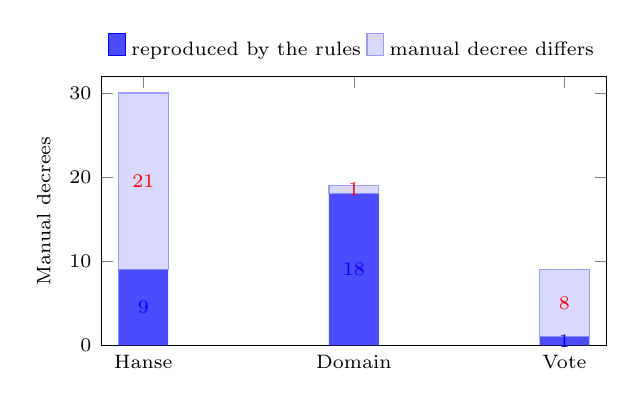
\begin{tikzpicture}
\begin{axis}[ybar stacked, width=8cm, height=5cm, bar width=18pt,
  symbolic x coords={Hanse,Domain,Vote}, xtick=data, ymin=0, ymax=32,
  ylabel={Manual decrees}, legend style={at={(0.5,1.02)},anchor=south,legend columns=2,draw=none,font=\scriptsize},
  tick label style={font=\scriptsize}, label style={font=\scriptsize}, nodes near coords, every node near coord/.append style={font=\scriptsize}]
\addplot+[fill=blue!70,draw=none] coordinates {(Hanse,9) (Domain,18) (Vote,1)};
\addplot+[fill=blue!15,draw=blue!40] coordinates {(Hanse,21) (Domain,1) (Vote,8)};
\legend{reproduced by the rules, manual decree differs}
\end{axis}
\end{tikzpicture}
\caption{Reproduction by rule. Where the Manual assigns a word by domain the engine agrees; where a word is shared or voted, the author's hand shows.}
\label{fig:rules}
\end{figure}

\paragraph{Classifying the divergences.} We read every divergent derivation trace and classified the cause (Table~\ref{tab:divergence}). Four classes account for all thirty.

\begin{enumerate}
\item \textbf{Hanse precedence (10).} The engine finds a skeleton shared by two families and inherits it; the Manual applied the Domain Rule instead. \emph{Cod}: Finnish \emph{turska}, Estonian \emph{tursk}, Swedish/Danish \emph{torsk}, Russian \emph{треска} all share T-R-S-K, so the engine takes the Hanse word (tie $\rightarrow$ Danish, \emph{torsk}); the Manual says ``Domain: Finnic (et)'' and gives \emph{tursk}. The same happens for \emph{water} (Lithuanian \emph{vanduo}, Danish \emph{vand}), \emph{winter} (Baltic \emph{ziema}, Slavic \emph{zima}), \emph{ice} (Baltic \emph{ledus}, Slavic \emph{lód}), \emph{sun} (Baltic \emph{saule}, Slavic \emph{solnce}, Germanic \emph{sol}), \emph{salmon}, \emph{cold}, \emph{sail} (Polish \emph{żeglować} is itself a Low German loan, sharing S-K-L with Swedish \emph{segla}), \emph{many} and \emph{Baltic herring}. In every case the Manual's form is the domain family's, and the domain family is Finnic nine times out of ten: the author, consciously or not, protected the sea vocabulary's Finnic character against the Hanse Rule. Whether Rule 1 or Rule 2 should have precedence for words that are both shared and domain-owned is a genuine design question the Manual's text answers one way and its examples another.
\item \textbf{Filling in a Hanse word (9).} Engine and Manual agree the word is shared and agree on the skeleton, but choose a different member's stem or a different vowel length: \emph{sild}/\emph{silk}, \emph{boot}/\emph{bot}, \emph{bu-}/\emph{buu-}, \emph{dzintar}/\emph{jantar}, \emph{tu}/\emph{du}, \emph{tri}/\emph{tre}, \emph{fem}/\emph{penki}, \emph{plav-}/\emph{pliv-}, \emph{kui}/\emph{än}. The Manual's stated procedure for this step (``family vote, ties by the Visby Queue'') underdetermines the outcome, and its own examples follow neither a whole-stem nor a position-wise vote consistently (\emph{boot} keeps the German long vowel; \emph{bu-} drops the Baltic one).
\item \textbf{Vote accounting and queue state (10).} For function words the engine's ballots or its queue state differ from the Manual's narrative. \emph{I}: the Manual counts Swedish \emph{jag} as skeleton J, discarding the final consonant, and finds J in two families; the engine reads J-K. \emph{Tomorrow}: the Manual reports a tie broken in Estonian's favour; the engine finds Germanic alone agreeing (\emph{imorgon}, \emph{i morgen}, \emph{morgen}) and lets it win outright. \emph{Question particle}: the Manual says every family abstained; the engine's one-differing-position tolerance lets Latvian \emph{vai} and Lithuanian \emph{ar} (V vs R) agree, so Baltic votes. \emph{And}: engine and Manual agree on the collision with \emph{ja} ``I'' but take a different runner-up. The remaining cases (\emph{we, you (pl.), one, no, very, but}) are of the same kind.
\item \textbf{Stem extraction (1).} \emph{See}, above.
\end{enumerate}

\begin{table}[t]
\centering\small
\caption{The thirty divergences by cause.}
\label{tab:divergence}
\begin{tabular}{@{}p{3.1cm}rp{3.7cm}@{}}
\toprule
Cause & $n$ & Items \\
\midrule
Manual applied Domain where a skeleton is shared & 10 & baltic-herring, many, water, sail, winter, ice, cod, salmon, sun, cold \\
Different fill-in of a shared skeleton & 9 & herring, boat, amber, be, you, three, five, swim, than \\
Vote accounting or queue state & 10 & I, we, you-pl, one, and, no, question, tomorrow, very, but \\
Stem extraction & 1 & see \\
\bottomrule
\end{tabular}
\end{table}

Two conclusions follow. First, the Manual is \emph{almost} an algorithm: the two rules that carry most of the semantic weight---who owns a domain, and which words are already shared---are reproduced, and the divergences sit in the last, least-specified step of filling in a shared form and in the bookkeeping of ballots. Second, the divergences are not random. They protect the Finnic character of sea vocabulary and prefer shorter, more Scandinavian-looking forms (\emph{sild} over \emph{silk}, \emph{fem} over \emph{penki}, \emph{tri} over \emph{tre}). This is exactly the editorial taste the design set out to remove, and the value of the exercise is that it can now be seen and argued about. The Manual remains authoritative for the seed lexicon (its forms are used, and the translator marks them ``manual decree''); the engine is authoritative for every word coined after it.

\paragraph{Sensitivity to the matching threshold.} The one interpretive decision with the largest effect is the length below which skeletons must match exactly (\S\ref{sec:skeleton}). Allowing one differing position at all lengths makes almost every short word a Hanse word: ``sea'' became a blend of \emph{meri}, \emph{mor} and \emph{juur} and reproduction fell to 16 of 58. Requiring exact matches for one- and two-consonant skeletons in Rule 1 raised it to 28. Extending the same restriction to family ballots in Rule 3 would fix the question particle but break \emph{many} (Latvian \emph{daudz} T-T and Lithuanian \emph{daug} T-K must agree for Baltic to vote, as the Manual says they do). We keep the Manual's wording for Rule 3 and record the tension.

\subsection{Reproducing the sentences}\label{sec:eval-sent}
We hand-wrote grammatical analyses (lemma, case, number, tense, person, order) for the Manual's twelve example sentences and the first sentence of its text, and rendered them with the engine using the seed lexicon. Twelve of thirteen come out verbatim, including all inflection, the head-final compound \emph{peleekhülje}, the copula, negation after the copula, the question particle, and every Repair the Manual illustrates (\emph{kaljuil, pospolitist, dužim, dužit, lääste, vidit, žeglisme}). The exception is \emph{bootse} ``in a boat'', which the Manual prints as \emph{bootise}: Rule 6 as the Manual states it does not insert a vowel into a two-consonant medial cluster (compare the Manual's own \emph{vidme}, \emph{vidte}), so we treat \emph{bootise} as a slip in the text rather than a rule. The full regular paradigm of \emph{vidte} (fifteen forms) and the copula (fifteen forms) are reproduced exactly; these paradigms were the decisive evidence for the boundary-sensitive formulation of epenthesis in \S\ref{sec:repair}.

\subsection{Determinism and stability}
The engine is a pure function of its inputs: 117 automated tests run on every change, covering the Normalization Table's examples, skeleton matching, citation stripping, every Repair example, the noun, adjective, pronoun and verb paradigms, the twelve sentences, reverse parsing, and the full lexicon reproduction, with the list of thirty divergences pinned so that any change in engine behaviour is visible as a test failure. The tie-break queue is an explicit, serialisable value; a derivation records the queue before and after, so any word's coining can be replayed and audited. In the deployed translator (\S\ref{sec:engine}) the derivation of new words was stable across repeated requests and across sessions by construction of the first-derivation-wins cache.

\section{The translation engine}\label{sec:engine}

A language no one has spoken needs a way to be spoken. We built a public translator between Baltmeri and the nine coastal languages (plus English as a pivot) whose defining property is that \emph{the language model never writes a Baltmeri word}. Figure~\ref{fig:arch} shows the architecture.

\begin{figure}[t]
\centering
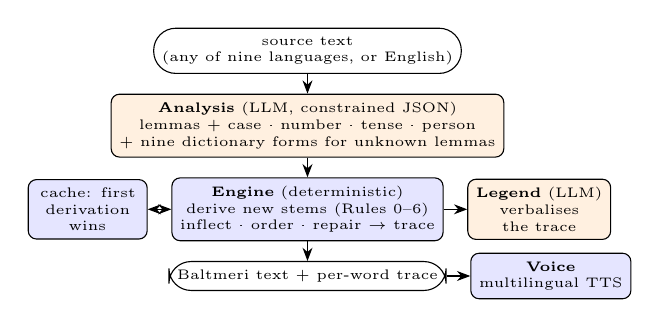
\begin{tikzpicture}[font=\tiny,node distance=2.5mm and 3mm,>=Stealth,
  llm/.style={draw,rounded corners=3pt,fill=orange!12,align=center,inner sep=3pt},
  det/.style={draw,rounded corners=3pt,fill=blue!10,align=center,inner sep=3pt},
  io/.style={draw,rounded corners=8pt,fill=white,align=center,inner sep=3pt}]
  \node[io] (src) {source text\\(any of nine languages, or English)};
  \node[llm,below=of src] (an) {\textbf{Analysis} (LLM, constrained JSON)\\lemmas + case · number · tense · person\\+ nine dictionary forms for unknown lemmas};
  \node[det,below=of an] (eng) {\textbf{Engine} (deterministic)\\derive new stems (Rules 0--6)\\inflect · order · repair $\rightarrow$ trace};
  \node[io,below=of eng] (out) {Baltmeri text + per-word trace};
  \node[llm,right=of eng] (leg) {\textbf{Legend} (LLM)\\verbalises\\the trace};
  \node[det,right=of out] (tts) {\textbf{Voice}\\multilingual TTS};
  \node[det,left=of eng,text width=1.3cm] (kv) {cache: first derivation wins};
  \draw[->] (src)--(an); \draw[->] (an)--(eng); \draw[->] (eng)--(out);
  \draw[->] (eng.east)--(leg.west); \draw[->] (out.east)--(tts.west);
  \draw[<->] (eng.west)--(kv.east);
\end{tikzpicture}
\caption{Architecture. Orange: probabilistic (language model); blue: deterministic. The model analyses and explains; the engine decides.}
\label{fig:arch}
\end{figure}

\subsection{Division of labour}
The design follows a line of work showing that large language models translate natural language into structured intermediate representations far more reliably than they execute the subsequent steps, and that delegating execution to a deterministic interpreter improves both accuracy and the faithfulness of explanations \citep{gao2023,lyu2023,pan2023,olausson2023,cheng2023}. The case is especially strong for morphology: wug-test studies find that language models ``massively underperform purpose-built systems'' at inflecting novel words, that success tracks community size and data availability rather than grammatical knowledge, and that even given a complete grammar book models apply rules only partially \citep{weissweiler2023,pantelidou2026,tanzer2024,bean2024}. A constructed language with no corpus is the worst case for such a model and the best case for a rule engine, whose ordered rewrite rules are total and predictable \citep{kaplan1994}. Corpus-based machine translation is simply unavailable: there is no parallel text \citep{nllb2024}.

\paragraph{Analysis.} The model receives the source text, a compact statement of Baltmeri syntax and case semantics, and the list of known lexicon identifiers. It returns, under a JSON schema enforced by constrained decoding \citep{willard2023,geng2023}, a sequence of word specifications---lemma, part of speech, case, number, degree, tense, person, compound and derivation flags---already in Baltmeri order, plus a \emph{newConcepts} list giving, for every lemma the engine does not know, the first dictionary translation in each of the nine languages in native orthography, a part of speech and a domain. This is an interlingua in the classical sense \citep{hutchins1992}, closest to the abstract syntax of Grammatical Framework \citep{ranta2011}, with the model in the role of the parser and the engine in the role of the concrete-syntax lineariser; the generation side is a rule pipeline of the Apertium kind \citep{forcada2011}. Following \citet{tam2024}, the format constraint is confined to the analysis payload; the model is never asked to reason inside the constrained call about how a word should be derived.

\paragraph{Derivation and rendering.} The engine starts a fresh queue from the canonical state, derives new concepts in order of first appearance, checks each form for collisions against the whole coined lexicon, inflects every word from the tables in \S\ref{sec:morphology}, inserts \emph{ne} and \emph{li}, capitalises and punctuates. Every token carries a trace: source forms, skeletons, rule, family, deciding language, queue before and after, repairs, and whether the form is a manual decree.

\paragraph{Legend.} A second model call receives the source, the Baltmeri and the trace, and writes the explanatory ``legend'' shown beneath the translation. Because it verbalises an executed trace rather than reasoning about the translation, the legend is faithful by construction in the sense of \citet{jacovi2020}; free-text self-explanations, by contrast, are known to misrepresent a model's actual process \citep{turpin2023}. The legend is instructed to say plainly where the Manual decreed a form over its own rules.

\paragraph{Reverse direction and voice.} Baltmeri to natural language runs the tables backwards: a parser indexes every inflected form of every known stem (about 40 forms per noun, 16 per verb), glosses each token with lemma and features, and the model renders the gloss into the target language with its own legend. Spoken output uses a multilingual neural voice with \emph{no language code}: Baltmeri is not a supported language, and since its orthography is a Finnic--Baltic--Slavic blend, forcing any single language's phonology would bias the accent.

\subsection{Deployment and behaviour}
The system runs as a single edge worker with a key--value store for the first-derivation-wins cache, analyses and legends. Typical latency is 7--11 seconds for a sentence, dominated by the analysis call. Figure~\ref{fig:ui} shows the interface on the Manual's second sentence. In use, the visible marking of new words (wavy underline) and manual decrees (in the trace) has proved to be the feature users engage with most: the language's accountability is its interface.

\begin{figure}[t]
\centering
\fbox{\parbox{0.93\linewidth}{\small\ttfamily
\textbf{Grey seals rest on the rocks in summer.}\\[2pt]
$\rightarrow$ Peleekhüljei odpočiv kaljuil suvil.\\[4pt]
\rmfamily\footnotesize
\textbf{Legend.} The sentence keeps its SVO shape, with place before time, and the two location words both end in \emph{-l}, the case that means ``on/at/when''. \emph{Peleekhüljei}: no skeleton was shared, so the Domain Rule stepped in: sea belongs to Finnic, Estonian ranks first, \emph{hüljes} $\rightarrow$ \emph{hülje}; the head-final compound \emph{peleek} + \emph{hülje}; \emph{-i} plural. \emph{odpočiv}: a verb of action, Slavic, Polish first: \emph{odpoczywać} $\rightarrow$ \emph{odpočiv}; third person takes a zero ending. \emph{kaljuil}: landscape is Finnic, Estonian \emph{kalju}; \emph{-i} plural, \emph{-l} on. \emph{suvil}: seasons are Finnic, Estonian \emph{suvi}; \emph{-l} here does its ``when'' duty. No Visby Queue tie-breaks were needed.}}
\caption{Translator output for the Manual's second sentence: the translation (main field) and the model-written legend grounded in the engine's trace.}
\label{fig:ui}
\end{figure}

\section{Discussion}\label{sec:discussion}

\subsection{What the divergences teach}
The reproducibility study is, to our knowledge, the first time a constructed language's founding text has been tested against its own stated procedure. The result---the Manual is an algorithm for what things mean and who owns them, and a hand for how they sound---is informative in both directions. It shows that determinism is achievable for the semantically loaded decisions: no reader of the Manual could complain that \emph{kala} or \emph{duž} or \emph{peleek} were chosen by taste. And it locates the residue of taste precisely, in the filling-in of shared words and the counting of ballots. A second edition of the Manual could close the gap in one of two ways: by adopting the engine's fully specified fill-in rule and accepting \emph{silk} and \emph{penki}, or by stating explicitly that the Domain Rule takes precedence for the sea vocabulary and that Hanse words keep the vowel length of the family that ranks first in the queue at the time of derivation. Either would make Baltmeri deterministic to the last letter; our recommendation is the first, because a language that belongs to the sea should not privilege how the sea sounds in Estonian.

\subsection{Equity, measured}
The family-balance result (Table~\ref{tab:balance}) is the design's central empirical claim. Germanic, with three members and roughly 110 million first-language speakers, supplies the fewest forms; Baltic, with two members and under five million speakers, supplies the most. This is not a bias toward the small: it is what happens when a shared word is counted once per family and when the tie-break geography is the sea's rather than the speaker count's. Interslavic's equal weighting of six sub-branches \citep{merunka2019} produced the same effect within one family; Baltmeri shows it can be produced across four. The obverse is that Latvian, by its early place in the queue, decided fourteen ties before the Rota Rule pushed it to the back; a language's influence in Baltmeri is a function of where its coast lies, which is the design's intention and its most contestable feature.

\subsection{The Baltic as a subject}
We began from the observation that the sea has no name of its own. Baltmeri gives it one, and a way of talking about itself in which \emph{Meri er men} ``the sea is ours'' means what a citizen of the Baltic would want it to mean: not possession but belonging. The legal and institutional turn toward recognising ecosystems as persons \citep{stone1972,teawatupua2017,spain2022,kauffman2021} requires guardians who speak for the entity; \citet{thiel2024} has proposed exactly such a body for this sea. A guardian who speaks \emph{for} a sea still speaks in a national language. A guardian who can also speak \emph{as} the sea---in a language generated from all its shores and owned by none---has something new to say, and the everyday users of a translator that shows its work are, in a small way, practising the bioregional citizenship Thiel describes. We do not claim that a constructed language will restore oxygen to the Gotland Deep. We claim that identity precedes care, that \citet{gotz2016} is right that Baltic identity has not followed Baltic institutions, and that a language is one of the few instruments---\citet{anderson2006} showed the print-language was the decisive one---by which a community can imagine itself into being. The environmental humanities have given us the words for a sea that is not outside us \citep{neimanis2017,steinberg2015,haraway2016}; Baltmeri is an attempt to give the sea words of its own.

\subsection{Limitations}
The nine ``first dictionary translations'' on which every derivation depends are a human or model judgement, and lexical choice upstream can change a word downstream: had we given Russian \emph{ходить под парусом} rather than \emph{плыть} for ``sail'', the ballot would differ. The Manual's queue is a convention that does not exactly track geography (\S\ref{sec:sources}); the choice of Saint Petersburg rather than Kaliningrad as Russia's coastal city is a political decision the text does not acknowledge. The seed lexicon is small and skewed toward the sea; a Leipzig--Jakarta list of core meanings \citep{tadmor2010} would be the natural next seed, and would test the procedure where families disagree most. The translator's analysis stage is probabilistic and can misanalyse a sentence even though every word it then receives is derived deterministically; the legend is faithful to the trace, not to the analysis. Baltmeri has no speakers, and intelligibility to speakers of the nine languages---the property Interslavic has measured at 84\%---has not been tested. Finally, the language is a proposition, not a claim on anyone: the nine languages of the shore are not diminished by a tenth that is made of them.

\subsection{Future work}
Three extensions follow directly. A crowd-sourced dictionary in which speakers of the nine languages supply and dispute source forms would make the upstream judgement communal rather than editorial, and would let the ``first derivation wins'' convention become a public record of who coined what. Cloze-based intelligibility studies on the Interslavic model would test whether Baltmeri is, as designed, passively readable around the sea. And a spoken form---the translator already voices Baltmeri with a multilingual model left to decide how it sounds---invites a phonetic study of what accent nine coastlines produce when no one is in charge.

\section{Conclusion}
Baltmeri is a language with a procedure where other languages have a history. Its words are decided by the nine languages of the Baltic shore voting as four equal families, with ties broken by the geography of the sea itself; its grammar is the set of endings those families could agree on; its lexicon can be extended by anyone with nine dictionaries and can be audited by anyone with the Manual. Implemented as a deterministic engine, the procedure reproduces the meaning-bearing decisions of its founding text and exposes, in the remaining half, exactly where a human hand intervened. Made usable through a translator in which a language model analyses and explains but never decides, it lets the citizens of the Baltic hear their sea say, in words that belong to all of them, \emph{meri er men}.

\section*{Data and code availability}
The Manual, the engine, the seed lexicon with all source forms, the 117 tests, and the translator are open source at \url{https://github.com/martinkallstrom/baltmeri-translator}. The translator is deployed at \url{https://baltmeri-translator.kindship-ai.workers.dev}. Every figure in \S\ref{sec:eval} is produced by scripts in the repository from the engine's own output.

\section*{Acknowledgements}
The authors thank the seals of Gotland for their patience.


\bibliographystyle{plainnat}
\small
\bibliography{refs}
\normalsize
\appendix
\section{The recipe card}\label{app:recipe}
To make any new Baltmeri word:
\begin{enumerate}\setlength{\itemsep}{1pt}
\item \textbf{Gather} the nine translations, normalize, strip endings, compute skeletons.
\item \textbf{Hanse check:} same skeleton in two families? Take it (family vote on the stem; ties by the queue).
\item \textbf{Content word?} Assign by domain (sea $\rightarrow$ Finnic, body/colour $\rightarrow$ Baltic, trade/abstract $\rightarrow$ Germanic, verbs/quality $\rightarrow$ Slavic); Estonian, Latvian, Polish, Swedish win inside their families.
\item \textbf{Function word or ending?} Family vote; ties by the Visby Queue; move the winner to the back.
\item \textbf{Nothing voted?} Fallback to the queue head that has a form.
\item \textbf{Collision?} The later concept takes its runner-up.
\item \textbf{Repair} clusters and add supporting \emph{-e}.
\item \textbf{Inflect:} plural \emph{-i}; cases \emph{-n, -a, -se, -l, -ste, -le}; verbs \emph{-u, -t, -Ø, -me, -te, -Ø}, past \emph{-l-}, future \emph{-s-}; negation \emph{ne}; question \emph{li}.
\end{enumerate}
To make a sentence: SVO, adjective before noun, place before time, no articles, no gender, stress the first syllable, and put the sea at the end.

\section{The seed lexicon with source forms}\label{app:lexicon}
Table~\ref{tab:lexicon} lists every seed entry in the Manual's derivation order with its nine source forms (fi · et · lv · lt · pl · ru · sv · da · de), the rule the engine applied (R1 Hanse, R2 Domain, R3 Vote), the winning family and deciding language, and whether the engine reproduces the Manual's decree (\checkmark) or the Manual decrees a different form ($\dagger$, engine form shown). Numerals six to ten have no manual decree.

\begin{table*}[p]
\centering\scriptsize
\caption{The seed lexicon.}
\label{tab:lexicon}
\setlength{\tabcolsep}{3pt}
\begin{tabular}{@{}llllllp{9.2cm}@{}}
\toprule
Gloss & Baltmeri & Engine & Rule & Family/by & & Sources (fi · et · lv · lt · pl · ru · sv · da · de) \tabularnewline
\midrule
sea & \textbf{meri} &  & R1 & Finnic/et & \checkmark & {\footnotesize meri · meri · jūra · jūra · morze · море · hav · hav · Meer} \tabularnewline
herring (Atlantic) & \textbf{sild} & silk & R1 & Baltic/lv & $\dagger$ & {\footnotesize silli · heeringas · siļķe · silkė · śledź · сельдь · sill · sild · Hering} \tabularnewline
sort, kind, variety & \textbf{sort} &  & R1 & Finnic/sv & \checkmark & {\footnotesize laji · sort · sorts · rūšis · sort · сорт · sort · sort · Sorte} \tabularnewline
salt & \textbf{sol} &  & R1 & Slavic/pl & \checkmark & {\footnotesize suola · sool · sāls · druska · sól · соль · salt · salt · Salz} \tabularnewline
boat & \textbf{boot} & bot & R1 & Germanic/sv & $\dagger$ & {\footnotesize vene · paat · laiva · laivas · łódź · лодка · båt · båd · Boot} \tabularnewline
amber & \textbf{dzintar} & jantar & R1 & Slavic/ru & $\dagger$ & {\footnotesize meripihka · merevaik · dzintars · gintaras · bursztyn · янтарь · bärnsten · rav · Bernstein} \tabularnewline
to be & \textbf{bu} & buu & R1 & Baltic/lt & $\dagger$ & {\footnotesize olla · olema · būt · būti · być · быть · vara · være · sein} \tabularnewline
fish & \textbf{kala} &  & R2 & Finnic/et & \checkmark & {\footnotesize kala · kala · zivs · žuvis · ryba · рыба · fisk · fisk · Fisch} \tabularnewline
Baltic herring & \textbf{räim} & silaka & R1 & Finnic/fi & $\dagger$ & {\footnotesize silakka · räim · {\stixfont reņģe} · strimelė · sałaka · салака · strömming · østersøsild · Strömling} \tabularnewline
seal & \textbf{hülje} &  & R2 & Finnic/et & \checkmark & {\footnotesize hylje · hüljes · ronis · ruonis · foka · тюлень · säl · sæl · Robbe} \tabularnewline
grey & \textbf{peleek} &  & R2 & Baltic/lv & \checkmark & {\footnotesize harmaa · hall · pelēks · pilkas · szary · серый · grå · grå · grau} \tabularnewline
big & \textbf{duž} &  & R2 & Slavic/pl & \checkmark & {\footnotesize suuri · suur · liels · didelis · duży · большой · stor · stor · groß} \tabularnewline
to rest & \textbf{odpočiv} &  & R2 & Slavic/pl & \checkmark & {\footnotesize levätä · puhkama · atpūsties · ilsėtis · odpoczywać · отдыхать · vila · hvile · ruhen} \tabularnewline
common & \textbf{pospolit} &  & R2 & Slavic/pl & \checkmark & {\footnotesize yleinen · tavaline · parasts · paprastas · pospolity · обычный · vanlig · almindelig · gewöhnlich} \tabularnewline
I & \textbf{ja} & es & R3 & Baltic/lv & $\dagger$ & {\footnotesize minä · mina · es · aš · ja · я · jag · jeg · ich} \tabularnewline
you (sg.) & \textbf{tu} & du & R1 & Germanic/de & $\dagger$ & {\footnotesize sinä · sina · tu · tu · ty · ты · du · du · du} \tabularnewline
he / she / it & \textbf{han} &  & R1 & Germanic/da & \checkmark & {\footnotesize hän · tema · viņš · jis · on · он · han · han · er} \tabularnewline
we & \textbf{me} & meie & R1 & Finnic/et & $\dagger$ & {\footnotesize me · meie · mēs · mes · my · мы · vi · vi · wir} \tabularnewline
you (pl.) & \textbf{juus} & teie & R3 & Finnic/et & $\dagger$ & {\footnotesize te · teie · jūs · jūs · wy · вы · ni · I · ihr} \tabularnewline
they & \textbf{de} &  & R3 & Germanic/sv & \checkmark & {\footnotesize he · nad · viņi · jie · oni · они · de · de · sie} \tabularnewline
one & \textbf{üks} & viens & R3 & Baltic/lv & $\dagger$ & {\footnotesize yksi · üks · viens · vienas · jeden · один · en · en · eins} \tabularnewline
two & \textbf{dva} &  & R1 & Slavic/pl & \checkmark & {\footnotesize kaksi · kaks · divi · du · dwa · два · två · to · zwei} \tabularnewline
three & \textbf{tri} & tre & R1 & Germanic/sv & $\dagger$ & {\footnotesize kolme · kolm · trīs · trys · trzy · три · tre · tre · drei} \tabularnewline
four & \textbf{četri} &  & R1 & Baltic/lv & \checkmark & {\footnotesize neljä · neli · četri · keturi · cztery · четыре · fyra · fire · vier} \tabularnewline
five & \textbf{fem} & penki & R1 & Baltic/lt & $\dagger$ & {\footnotesize viisi · viis · pieci · penki · pięć · пять · fem · fem · fünf} \tabularnewline
six & \textbf{seši} &  & R3 & Baltic/lv & — & {\footnotesize kuusi · kuus · seši · šeši · sześć · шесть · sex · seks · sechs} \tabularnewline
seven & \textbf{septini} &  & R3 & Baltic/lv & — & {\footnotesize seitsemän · seitse · septiņi · septyni · siedem · семь · sju · syv · sieben} \tabularnewline
eight & \textbf{ota} &  & R3 & Germanic/sv & — & {\footnotesize kahdeksan · kaheksa · astoņi · aštuoni · osiem · восемь · åtta · otte · acht} \tabularnewline
nine & \textbf{dzevents} &  & R3 & Slavic/pl & — & {\footnotesize yhdeksän · üheksa · deviņi · devyni · dziewięć · девять · nio · ni · neun} \tabularnewline
ten & \textbf{desmit} &  & R1 & Baltic/lv & — & {\footnotesize kymmenen · kümme · desmit · dešimt · dziesięć · десять · tio · ti · zehn} \tabularnewline
and & \textbf{i} & un & R3 & Baltic/lv & $\dagger$ & {\footnotesize ja · ja · un · ir · i · и · och · og · und} \tabularnewline
not & \textbf{ne} &  & R1 & Baltic/lv & \checkmark & {\footnotesize ei · ei · ne · ne · nie · не · inte · ikke · nicht} \tabularnewline
no (answer) & \textbf{nei} & nee & R1 & Baltic/lt & $\dagger$ & {\footnotesize ei · ei · nē · ne · nie · нет · nej · nej · nein} \tabularnewline
(yes/no question particle) & \textbf{li} & vai & R3 & Baltic/lv & $\dagger$ & {\footnotesize — · kas · vai · ar · czy · ли · — · — · —} \tabularnewline
many & \textbf{daug} & mnogo & R1 & Slavic/ru & $\dagger$ & {\footnotesize monta · palju · daudz · daug · wiele · много · många · mange · viele} \tabularnewline
rock, cliff & \textbf{kalju} &  & R1 & Finnic/et & \checkmark & {\footnotesize kallio · kalju · klints · uola · skała · скала · klippa · klippe · Felsen} \tabularnewline
summer & \textbf{suvi} &  & R2 & Finnic/et & \checkmark & {\footnotesize kesä · suvi · vasara · vasara · lato · лето · sommar · sommer · Sommer} \tabularnewline
to see & \textbf{vid} & vidz & R2 & Slavic/pl & $\dagger$ & {\footnotesize nähdä · nägema · redzēt · matyti · widzieć · видеть · se · se · sehen} \tabularnewline
water & \textbf{vesi} & vand & R1 & Baltic/lt & $\dagger$ & {\footnotesize vesi · vesi · ūdens · vanduo · woda · вода · vatten · vand · Wasser} \tabularnewline
to love & \textbf{koh} &  & R2 & Slavic/pl & \checkmark & {\footnotesize rakastaa · armastama · mīlēt · mylėti · kochać · любить · älska · elske · lieben} \tabularnewline
to catch & \textbf{lov} &  & R2 & Slavic/pl & \checkmark & {\footnotesize pyydystää · püüdma · ķert · gaudyti · łowić · ловить · fånga · fange · fangen} \tabularnewline
autumn & \textbf{sügis} &  & R2 & Finnic/et & \checkmark & {\footnotesize syksy · sügis · rudens · ruduo · jesień · осень · höst · efterår · Herbst} \tabularnewline
yesterday & \textbf{vakar} &  & R1 & Baltic/lv & \checkmark & {\footnotesize eilen · eile · vakar · vakar · wczoraj · вчера · igår · i går · gestern} \tabularnewline
tomorrow & \textbf{home} & imorgon & R3 & Germanic/sv & $\dagger$ & {\footnotesize huomenna · homme · rīt · rytoj · jutro · завтра · imorgon · i morgen · morgen} \tabularnewline
to sail & \textbf{žegl} & segl & R1 & Germanic/sv & $\dagger$ & {\footnotesize purjehtia · purjetama · burāt · buriuoti · żeglować · плыть · segla · sejle · segeln} \tabularnewline
wind & \textbf{tuul} &  & R2 & Finnic/et & \checkmark & {\footnotesize tuuli · tuul · vējš · vėjas · wiatr · ветер · vind · vind · Wind} \tabularnewline
to blow (wind) & \textbf{vi} &  & R2 & Slavic/pl & \checkmark & {\footnotesize tuulla · puhuma · pūst · pūsti · wiać · веять · blåsa · blæse · wehen} \tabularnewline
west & \textbf{lääs} &  & R2 & Finnic/et & \checkmark & {\footnotesize länsi · lääs · rietumi · vakarai · zachód · запад · väster · vest · Westen} \tabularnewline
to swim & \textbf{plav} & pliv & R1 & Slavic/pl & $\dagger$ & {\footnotesize uida · ujuma · peldēt · plaukti · pływać · плавать · simma · svømme · schwimmen} \tabularnewline
winter & \textbf{talv} & zim & R1 & Slavic/ru & $\dagger$ & {\footnotesize talvi · talv · ziema · žiema · zima · зима · vinter · vinter · Winter} \tabularnewline
small & \textbf{mal} &  & R2 & Slavic/pl & \checkmark & {\footnotesize pieni · väike · mazs · mažas · mały · малый · liten · lille · klein} \tabularnewline
than & \textbf{kui} & än & R1 & Baltic/lt & $\dagger$ & {\footnotesize kuin · kui · nekā · nei · niż · чем · än · end · als} \tabularnewline
deep & \textbf{glembok} &  & R2 & Slavic/pl & \checkmark & {\footnotesize syvä · sügav · dziļš · gilus · głęboki · глубокий · djup · dyb · tief} \tabularnewline
very & \textbf{müket} & loti & R3 & Baltic/lv & $\dagger$ & {\footnotesize hyvin · väga · ļoti · labai · bardzo · очень · mycket · meget · sehr} \tabularnewline
ice & \textbf{jää} & lod & R1 & Slavic/pl & $\dagger$ & {\footnotesize jää · jää · ledus · ledas · lód · лёд · is · is · Eis} \tabularnewline
cod & \textbf{tursk} & torsk & R1 & Germanic/da & $\dagger$ & {\footnotesize turska · tursk · menca · menkė · dorsz · треска · torsk · torsk · Dorsch} \tabularnewline
salmon & \textbf{lohi} & laks & R1 & Germanic/sv & $\dagger$ & {\footnotesize lohi · lõhe · lasis · lašiša · łosoś · лосось · lax · laks · Lachs} \tabularnewline
to live & \textbf{ži} &  & R2 & Slavic/pl & \checkmark & {\footnotesize elää · elama · dzīvot · gyventi · żyć · жить · leva · leve · leben} \tabularnewline
island & \textbf{saar} &  & R2 & Finnic/et & \checkmark & {\footnotesize saari · saar · sala · sala · wyspa · остров · ö · ø · Insel} \tabularnewline
sun, day & \textbf{päive} & saul & R1 & Baltic/lt & $\dagger$ & {\footnotesize päivä · päev · saule · saulė · słońce · солнце · sol · sol · Sonne} \tabularnewline
shore & \textbf{rand} &  & R2 & Finnic/et & \checkmark & {\footnotesize ranta · rand · krasts · krantas · brzeg · берег · strand · strand · Strand} \tabularnewline
cold & \textbf{zimne} & külm & R1 & Finnic/et & $\dagger$ & {\footnotesize kylmä · külm · auksts · šaltas · zimny · холодный · kall · kold · kalt} \tabularnewline
but & \textbf{ale} & bet & R3 & Baltic/lv & $\dagger$ & {\footnotesize mutta · aga · bet · bet · ale · но · men · men · aber} \tabularnewline
\bottomrule
\end{tabular}

\end{table*}

Derived entries: \emph{dužus} ``size'' (\emph{duž} + \emph{-us}), \emph{kalaja} ``fisher'' and \emph{žeglja} ``sailor'' (\emph{-ja}), \emph{kalaka} ``little fish'' (\emph{-ka}), \emph{solne} ``salty'' (\emph{-ne}); fixed: \emph{Baltmeri}.

\section{The interlingua}\label{app:interlingua}
The analysis stage of the translator (\S\ref{sec:engine}) returns a sequence of word specifications in Baltmeri order, each of one of the kinds in Table~\ref{tab:interlingua}, together with sentence-level flags \texttt{negated} and \texttt{question}, and a list of \emph{new concepts}: for every lemma outside the lexicon, its part of speech, semantic domain (Table~\ref{tab:domains}) and first dictionary translation in each of the nine languages in native orthography. Lemmas are English identifiers; the engine resolves them against the seed lexicon, the cache of previously coined words, and finally the new-concept list. The specification is deliberately shallow: it names what is to be said and with which grammatical features, and leaves every decision about form to the engine.

\begin{center}\small
\captionof{table}{Word specifications in the interlingua.}
\label{tab:interlingua}
\begin{tabular}{@{}lp{5.3cm}@{}}
\toprule
Kind & Features \\
\midrule
noun & lemma; number (sg, pl); case (nom, gen, acc, ine, ade, ela, all); optional compound modifier; optional derivation (abstract, agent, diminutive, adjective) \\
adj & lemma; number; degree (pos, comp, sup) \\
adv & lemma; whether formed from an adjective (\emph{-t}) \\
verb & lemma; tense (pres, past, fut); person (1, 2, 3); number; infinitive flag \\
pron & one of I, you, he, we, you-pl, they; case \\
num & numeric value (one to ten are words, larger values digits) \\
word & lemma of a conjunction, particle, quantifier or preposition \\
name & proper name in Latin script; case; number \\
punct & a punctuation mark inside the sentence \\
\bottomrule
\end{tabular}
\end{center}

For the sentence ``Grey seals rest on the rocks in summer'' the analysis is: \texttt{noun}(seal, pl, nom, compound grey) · \texttt{verb}(rest, pres, 3, pl) · \texttt{noun}(rock, pl, ade) · \texttt{noun}(summer, sg, ade), with no new concepts, from which the engine renders \emph{Peleekhüljei odpočiv kaljuil suvil}.

\end{document}
